\chapter{مروری بر مطالعات گذشته}

\section{مقدمه}
تولید خودکار شرح بر تصاویر، یکی از چالشی‌ترین مسائل روز در حوزه هوش مصنوعی به شمار می‌رود. در فصل گذشته، سیر پژوهش‌های انجام شده در این حوزه را به طور اجمالی مورد بررسی قرار دادیم. در این فصل، نگاه موشکافانه‌تری بر پژوهش‌های پیشین انداخته و چالش‌های مطرح‌شده و روند رفع هر یک از آن‌ها را به طور دقیق‌تر و با جزئیات بیشتر مورد بررسی قرار می‌دهیم.
\\
همانند بسیاری دیگر از مسائل مطرح در زمینه‌ هوش مصنوعی، ایده‌های اولیه برای حل مساله تولید خودکار شرح بر تصاویر نیز با بررسی عمل‌کرد مغز انسان، ایجاد شد. در بخش اول از این فصل، یکی از پژوهش‌هایی را که با هدف بررسی روند درک صحنه و توصیف تصویر توسط مغز انسان انجام شده را مورد بررسی قرار می‌دهیم تا با ویژگی‌های اصلی مورد انتظار برای چنین سامانه‌ای آشنا شویم.
\\
همان‌طور که گفته شد، فرایندهای تولید خودکار شرح بر تصاویر، در سال‌های قبل از 2014، عموما با هدف حل یکی از چالش‌های درک صحنه یا تولید جمله انجام می‌شدند. در ادامه بحث و بررسی پیرامون مطالعات گذشته، ابتدا نمونه‌هایی از روش‌های ارائه شده برای حل چالش درک صحنه و سپس نمونه‌هایی از پژوهش‌های انجام شده برای حل چالش تولید جمله را مورد بررسی قرار می‌دهیم.
\\
استفاده از شبکه‌های عصبی و یادگیری عمیق، که از سال‌های ۲۰۱۴ به بعد توجه تعداد زیادی از پژوهش‌گران را به خود جلب کرد، در ادامه این فصل مورد بررسی قرار می‌گیرد. روش‌های ارائه شده بر بستر کاری رمزگذار-رمزگشا و روند پژوهش با استفاده از این بستر کاری، به طور دقیق‌تر و با ارائه جزئیات بیش‌تر مورد مطالعه قرار خواهد گرفت. از آن‌جا که پژوهش حاضر، از این بستر کاری به عنوان چارچوب اصلی استفاده کرده است، تمرکز بحث در این قسمت، بیش از سایر قسمت‌ها خواهد بود.

\section{پژوهش‌های انجام‌شده در زمینه درک صحنه توسط مغز انسان}
مساله درک صحنه، مانند بیشتر مسائل موجود در زمینه بینایی ماشین، الهام گرفته از نحوه رفتار انسان‌ها است. اغلب انسان‌ها با دیدن یک تصویر قادرند توصیف کامل و دقیقی از آن تصویر ارائه دهند که شامل تمام نکات لازم و ضروری نهفته در تصویر باشد. در بیشتر موارد، زمان مورد نیاز برای مغز انسان به منظور پردازش یک تصویر و توصیف آن، زمان بسیار کم و ناچیزی است. این واقعیت، این ایده را در ذهن تداعی می‌کند که بخش قابل توجهی از اطلاعات مورد نیاز از هر تصویر، در اولین لحظاتی که تصویر به مغز می‌رسد (در نگاه اول) قابل استخراج است. بنابراین سامانه‌های رایانه‌ای باید قادر باشند با الگو گرفتن از مغز انسان، در کوتاه‌ترین زمان ممکن، اطلاعات کافی و مفید نهفته در تصویر را استخراج کرده و صحنه به نمایش کشیده شده در تصویر را توصیف کنند.
\\
این فرض که مغز انسان می‌تواند در کوتاه‌ترین زمان ممکن، بیشترین حجم اطلاعات تصویر را به درستی استخراج نماید، توسط پژوهش‌گران متعددی مورد ارزیابی قرار گرفته است. از جمله اولین پژوهش‌هایی که به بررسی این فرض پرداخته‌اند می‌توان به پژوهش‌های 
\cite{potter1976short}
و
\cite{potter2002recognition}
اشاره کرد. در این‌ پژوهش‌ها، با نشان دادن تصاویر به صورت دنباله‌ای\enfootnote{Image Series} به مجموعه‌ای از افراد، از آن‌ها خواسته شده تا بهترین و دقیق‌ترین توصیفی را که می‌توانند، برای تصاویری که دیده‌اند، بازگو کنند. نتایج حاصل از این دو پژوهش نشان می‌دهند که انسان می‌تواند یک تصویر معمولی را در بازه زمانی کمتر از ۲۰۰ میلی‌ثانیه، تشخیص داده و آن را توصیف کند. اگرچه این زمان برای تشخیص و توصیف یک تصویر کافیست، زمان مورد نیاز برای به‌خاطرسپاری تصویر بسیار بیشتر از این مقدار است.
\\
در پژوهش\cite{fei2007we}
آزمایش دیگری انجام شده که از اهمیت بسیاری برخوردار است. در پژوهش‌های قبلی، افرادی که تصاویر را توصیف می‌کردند، درباره موضوع کلی تصاویر اطلاعاتی داشتند. اما در این آزمایش، تصاویر مختلفی از دنیای واقعی که محدود به شرایط خاصی نبوده‌اند، بدون ارائه پیش‌فرض درباره موضوع، به افراد نمایش داده شده و از آن‌ها خواسته شده که تصویر را به بهترین شکل توصیف کنند. آزمایشات در این پژوهش، در دو مرحله انجام شده‌اند.
\begin{enumerate}
	\item توسط یک رایانه، تصاویر متعددی در بازه‌های زمانی متفاوت به افراد نمایش داده می‌شوند و پس از اتمام زمان نمایش هر تصویر، یک ماسک بصری، تصویر را می‌پوشاند. در این حالت از افراد خواسته‌شده  است که بهترین توصیف ممکن از تصویر را تایپ کنند. شرایط محیطی آزمایشات مطابق با استانداردها رعایت شده است. هر تصویر به طور تصادفی بین 27 الی 500 میلی ثانیه روی نمایش‌گر نمایش‌داده شده و سپس یک ماسک روی تصویرقرار گرفته و افراد فرصت دارند تا توصیف خود را از تصویر، بنویسند.
	
	
	\begin{figure}[h]
		\center
		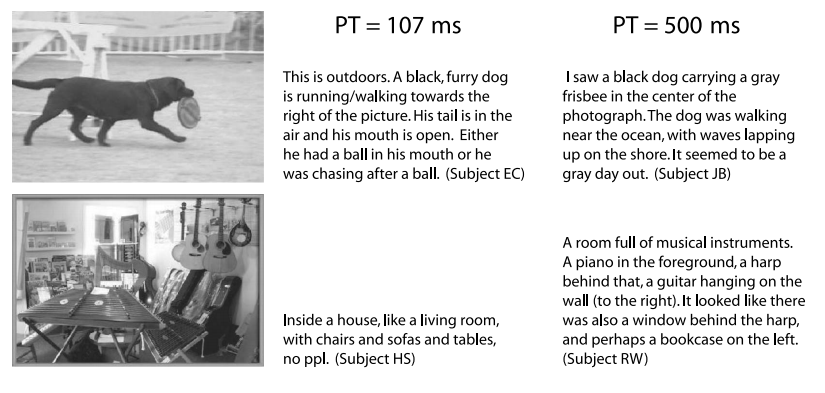
\includegraphics[scale=0.5]{./Imgs/fei2007we_res2.png}
		\caption[نمونه توصیف‌های افراد برای تصاویر]{نمونه‌ توصیف‌های افراد برای تصاویر\cite{fei2007we}}
		\label{fig:f2007we1}
	\end{figure}
	
	
	
	\item در این مرحله، آزمایش روی افراد متفاوتی انجام شده‌است. این گروه افراد موظفند پس از دیدن تصاویر، به بهترین شکل ممکن آن‌ها را دسته‌بندی کنند. برخلاف افراد شرکت‌کننده در آزمایش قبلی  که می‌توانستند به هر شکلی اطلاعات استخراج شده را بنویسند، به افراد حاضر در این گروه یک فرم مشخص از دسته‌اطلاعات مطلوب داده شده است که افراد موظفند آن را براساس محتوای تصویری که دیده‌اند، پر کنند. شکل\ref{fig:f2007we2}
	ساختار مطلوب پاسخ افراد را در این آزمایش نمایش می‌دهد.
	
	\begin{figure}[h]
		\center
		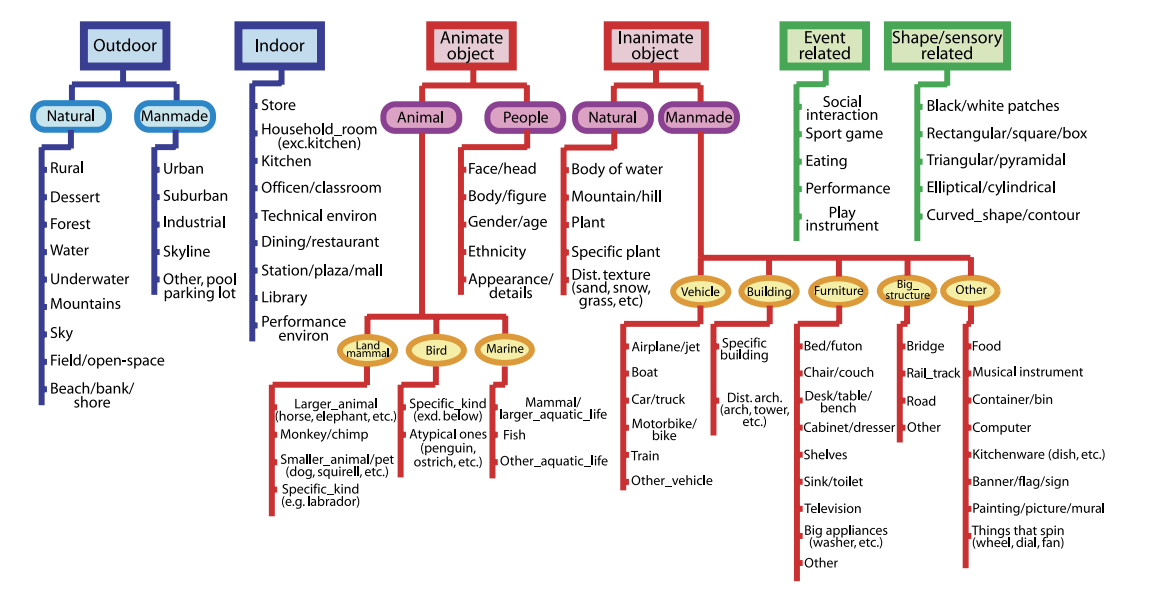
\includegraphics[scale=0.4]{./Imgs/fei2007we_exp1.png}
		\caption{ساختار مطلوب اطلاعات استخراج‌شده از تصاویر\cite{fei2007we}}
		\label{fig:f2007we2}
	\end{figure}
	
	این ساختار با تحلیل پاسخ‌های جمع‌آوری شده از آزمایش اول استخراج شده است و شامل انواع مختلفی از اطلاعات است که افراد در آزمایش اول به آن اشاره‌کرده‌اند.
	
	
	
	
	
\end{enumerate}


شکل\ref{fig:f2007wd}
چند نمونه از تصاویر مورد استفاده در آزمایشات این پژوهش را نمایش می‌دهد. این تصاویر از اینترنت استخراج شده‌اند. برای استخراج این تصاویر از فضای اینترنت، از یک گروه افراد شامل ۱۰ نفر که با موضوع پژوهش آشنا نبوده‌اند خواسته‌شده تا هر یک، نام ۵ دسته صحنه مختلف را به طور تصادفی بنویسند. پس از حذف نام‌های تکراری، ۲۵ الی ۳۰ نام منحصربه‌فرد باقی مانده‌است. سپس تصاویر مربوط به هریک از این نام‌ها توسط موتور جستجوی گوگل استخراج شده و ۳ الی ۶ تصویر از صفحات اولیه نتایج به عنوان تصاویر نمونه انتخاب شده‌اند.

\begin{figure}[h]
	\centering
	\begin{subfigure}[چند نمونه از تصاویر در محیط باز]{ 0.4\textwidth}
		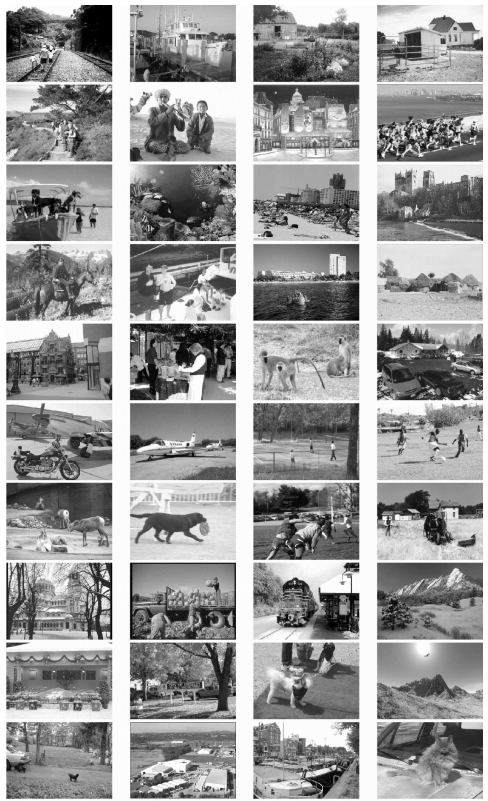
\includegraphics[scale=0.4]{Imgs/fei2007we_data1.png}
	\end{subfigure}
	\hfill
	\begin{subfigure}[چند نمونه از تصاویر در محیط بسته]{0.4\textwidth}
		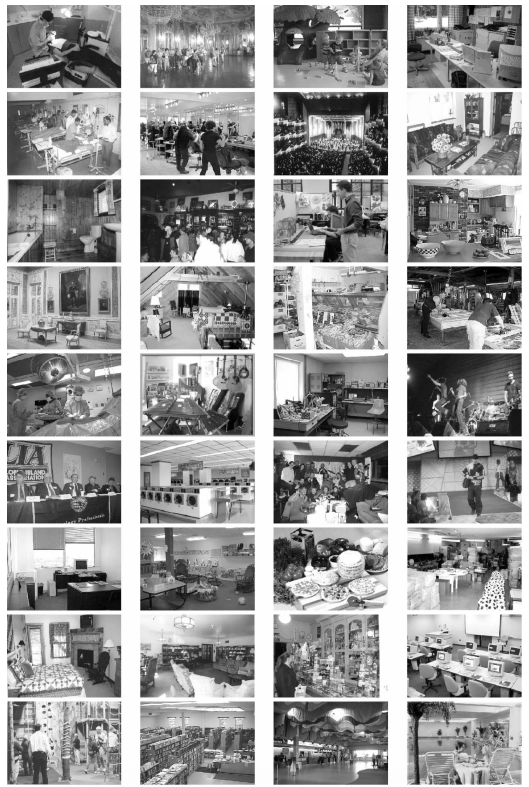
\includegraphics[scale=0.4]{Imgs/fei2007we_data2.png}
	\end{subfigure}
	\caption{تصاویر دنیای واقعی مورد استفاده در آزمایشات\cite{fei2007we}}
	\label{fig:f2007wd}
\end{figure}


ارزشمندترین نکته درباره پژوهش انجام‌شده، یافته‌های آن است. این پژوهش نکاتی را در مورد توانایی مغز انسان در توصیف صحنه روشن می‌کند که حائز اهمیت هستند. در ادامه این نتایج را بررسی خواهیم کرد.
\subsubsection{نتایج به‌دست‌ آمده از آزمایشات}
\begin{enumerate}
	\item
	حداکثر زمان لازم برای مغز انسان به منظور درک صحنه، برابر با 500 میلی‌ثانیه است.
	\item
	این مدت زمان، برای صحنه‌های ساده‌ و بدون پیچیدگی، به حدود ۱۰۰ میلی‌ثانیه می‌رسد. به عنوان نمونه در شکل\ref{fig:f2007we1} تصویر اول که دارای پیچیدگی‌های کمتری نسبت به تصویر دوم است در مدت زمان ۱۰۷ میلی‌ثانیه، به‌طور کامل توصیف شده‌است در صورتی‌که تصویر دوم که به نسبت، پیچیده‌تر است، مدت‌زمان بیشتری برای توصیف نیاز داشته‌است.
	\item
	با استفاده از ساختارمندسازی پاسخ‌های افراد در آزمایش دوم و اطلاعات جمع‌آوری شده در درخت پاسخ‌ها (که در شکل\ref{fig:f2007we2} نمایش‌ داده شده است) و میانگین‌گیری روی تمام تصاویر، نمودارهای مقایسه‌ای برای مدت زمان 107 میلی‌ثانیه و 500 میلی‌ثانیه ایجاد شده‌ است. شکل\ref{fig:f2007res3}
	نمودارهای مقایسه‌ای را نمایش‌ می‌دهد. در این نمودارها، میله‌های قرمز نشان‌دهنده نتایج برای زمان ۵۰۰ میلی‌ثانیه و میله‌های آبی نمایش‌دهنده نتایج برای حالت ۱۰۷ میلی‌ثانیه هستند.
	در دو نمودار اول (نمودارهای بالا سمت راست و بالا سمت چپ) تشخیص و استخراج اطلاعات مربوط به اجسام مختلف بسته به متحرک بودن\enfootnote{Animated} یا متحرک نبودن\enfootnote{Inanimated} آن‌ها، در نمودار سوم (نمودار پایین سمت چپ) تشخیص و استخراج اطلاعات مربوط به صحنه موجود در تصویر و در نمودار چهارم‌ (نمودار پایین سمت راست) تشخیص و استخراج اطلاعات مربوط به رخداد موجود در تصویر، مورد بررسی قرار گرفته‌اند.
	
	
	\begin{figure}[h]
		\center
		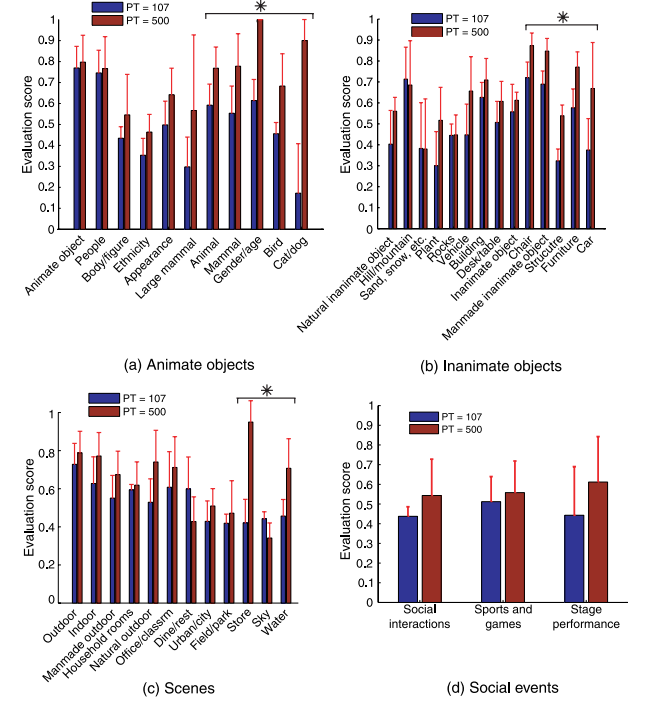
\includegraphics[scale=0.6]{./Imgs/fei2007we_res3.png}
		\caption[نمودار مقایسه‌ای عملکرد مغز در درک صحنه]{نمودارهای مقایسه‌ای عملکرد مغز انسان در درک صحنه در بازه‌های زمانی ۱۰۷ و ۵۰۰ میلی‌ثانیه\cite{fei2007we}}
		\label{fig:f2007res3}
	\end{figure}
	
	همان‌طور که مشخص است، مدت زمان ۱۰۷ میلی‌ثانیه برای مغز انسان، زمان بهینه برای توصیف صحنه است. تفاوت‌های بین نتایج در اکثر موارد، جزئی و در مقابل تفاوت زمانی موجود، بسیار کوچک هستند.
	به علاوه، در تمام مواردی که نیاز به اطلاعات کلی از تصویر وجود دارد، تفاوت بین دو بازه زمانی چندان چشم‌گیر نیست، اما در مواردی که برای تشخیص نیاز به دانستن جزئیات بیشتر از تصویر وجود دارد (مانند سن، جنسیت و نوع حیوان) تفاوت بین دو زمان، قابل ملاحظه است.
	\\
	همین‌طور با مقایسه تفاوت عملکرد بین حالات متحرک بودن و متحرک نبودن اجسام، فواصل موجود در نمودارها قابل ملاحظه می‌شود. در حالت کلی، تفاوت بین عملکرد مغز در دو بازه، در حالتی‌که اجسام ساکن در تصویر وجود دارند به مراتب کمتر از حالتی است که اجسام موجود در تصویر، متحرک باشند.
\end{enumerate}

شکل\ref{fig:f2007res4} نمونه دیگری از نتایج به‌دست‌آمده از آزمایشات را در مدت‌زمان‌های مختلف نمایش ‌می‌دهد. در این شکل، سه تصویر از مجموعه تصاویر انتخاب شده و با مدت‌زمان‌های مختلف، به افراد نمایش داده شده است. در این شکل، نمونه‌هایی از توصیفات تولید شده توسط انسان، برای هر یک از تصاویر و در زمان‌های مختلف قابل مشاهده هستند.



\begin{figure}[h]
	\center
	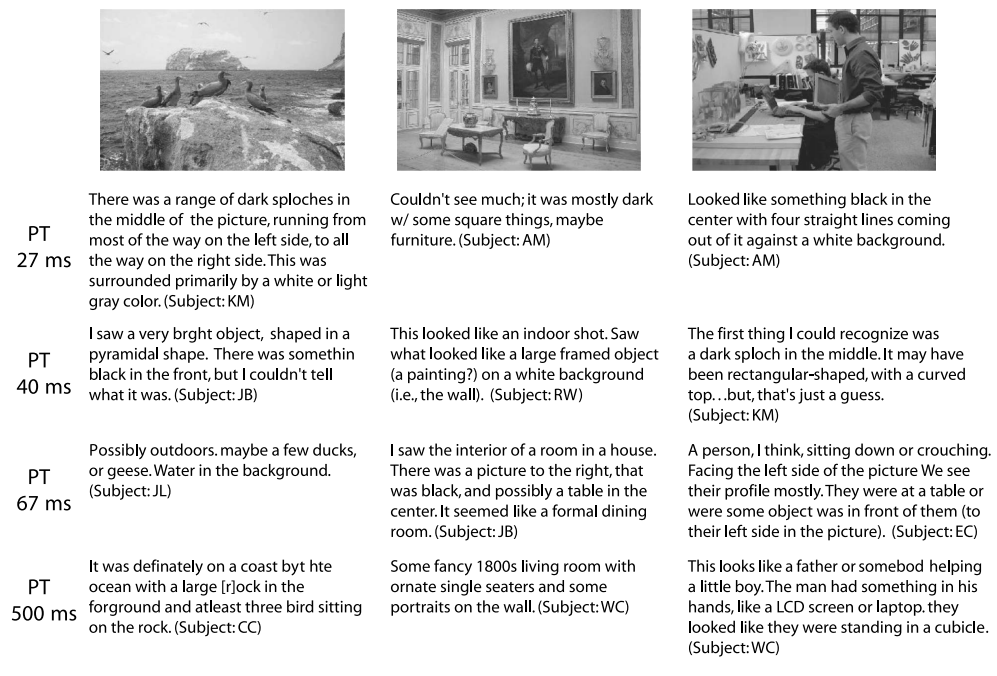
\includegraphics[scale=0.4]{./Imgs/fei2007we_res4.png}
	\caption{نمونه‌ای از نتایج به‌دست‌آمده از آزمایشات\cite{fei2007we}}
	\label{fig:f2007res4}
\end{figure}

%%%%%%%%%%%%%%%%%%%%%%%%%%%%%%%%%%%%%%%%%
\section{روش‌های مبتنی بر مدل‌های گرافی-احتمالی}

همان‌طور که قبلا ذکر شد، روش‌های مبتنی بر استفاده از مدل‌های گرافی احتمالی، از جمله پرکاربردترین روش‌ها در مرحله درک صحنه در زمینه تولید خودکار شرح بر تصاویر هستند. این روش‌ها با استفاده از نظریه گراف، آمار و احتمالات اقدام به ارائه یک توزیع احتمالی برای متغیر تصادفی مورد بررسی، با توجه به داده‌های موجود در مجموعه آموزشی می‌کنند. تا کنون، مدل‌های استاندارد گرافی-احتمالی مختلفی برای حل مسائل مختلف، ارائه شده‌اند که تقریبا از تمام این مدل‌ها می‌توان در بخش‌های مختلف تولید شرح خودکار بر تصاویر، استفاده نمود. یک نمونه از کاربرد مدل میدان تصادفی مارکف، یک نمونه از کاربر مدل میدان تصادفی شرطی و یک نمونه از کاربرد یک مدل مولد خاص‌منظوره، که توسط خانم لی و همکارانش طراحی شده است، در مساله تولید خودکار شرح بر تصاویر را مورد بررسی قرار می‌دهیم.

\subsection[استفاده از مدل میدان تصادفی مارکف]{استفاده از مدل میدان تصادفی مارکف\enfootnote{Markov Random Field (MRF)}\cite{Farhadi2010every}}
پژوهش 
\cite{Farhadi2010every}
که توسط آقای فرهادی و همکارانش در سال 2010 انجام شده است، با استفاده از یک مدل ساده میدان تصادفی مارکف، به حل مساله درک صحنه می‌پردازد. مدل ارائه شده در این پژوهش، علاوه بر حل چالش درک صحنه، تا حدودی می‌تواند برای تولید جملات توصیف‌گر تصویر نیز مورد استفاده قرار بگیرد.
\\
همان‌طور که قبلا ذکر شد، اطلاعات قابل استخراج در فرایند درک صحنه، در هر پژوهش بسته به کاربرد و علاقه پژوهش‌گران، قابل تعریف است. در پژوهش \cite{Farhadi2010every} اطلاعات قابل استخراج از تصویر شامل موارد زیر می‌شود:
\begin{enumerate}
	\item اجسام موجود
	\item فعالیت به تصویر کشیده شده
	\item صحنه موجود
\end{enumerate}
بنابر تعریف فوق، در فرایند درک صحنه در این پژوهش، به ازای هر تصویر، یک سه‌تایی «جسم، فعالیت، صحنه»\enfootnote{<Object, Activity, Scene>}
ایجاد می‌شود که بیان‌کننده اطلاعات مطلوب موجود در تصویر است. مولفه\enfootnote{Field} «جسم» در این سه‌تایی، مشخص‌کننده‌ برچسب حاصل از دسته‌بندی اجسام موجود در صحنه، مولفه «فعالیت»، مشخص‌کننده اطلاعات مربوط به فعالیت در حال انجام و مولفه «صحنه»، مشخص‌کننده اطلاعات مربوط به محیط تصویر هستند. از آن‌جایی که هر سه‌تایی مربوط به یک تصویر، محتوای تصویر را توصیف می‌نماید، به فضای این سه‌تایی‌ها، فضای معنا\enfootnote{Meaning Space} می‌گویند.
\\
شکل
\ref{fig:F2010EF1}
نمایی از نگاشت اطلاعات از فضای تصاویر و جملات به فضای معنایی، نمایش می‌دهد. همان‌طور که در شکل مشخص است، به ازای هر تصویر، یک سه‌تایی معنایی ایجاد می‌شود. همین‌طور به ازای هر جمله در فضای جملات، یک سه‌تایی ایجاد می‌شود به‌طوری‌که جملات و تصاویر متناظرشان، به یک سه‌تایی یکسان، نگاشت شوند. همان‌طور که مشخص است، با داشتن نگاشت‌هایی  که خواص مذکور را داشته‌باشند، می‌توان با استفاده از سه‌تایی‌های فضای معنا، تصاویر را مدیریت کرد.

\begin{figure}[h]
	\center
	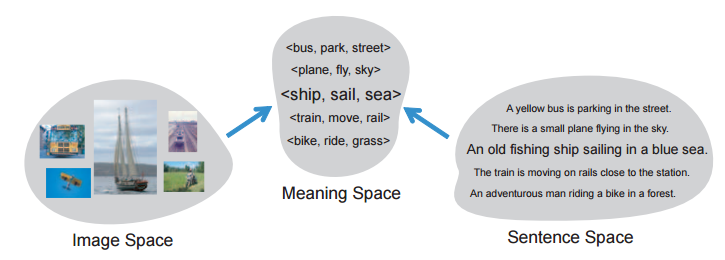
\includegraphics[scale=0.6]{./Imgs/farhadi2010every_fig1.png}
	\caption[نگاشت تصویر به فضای معنایی]{
		نگاشت تصویر به فضای معنایی. فضای معنایی شامل اطلاعات مطلوب برای استخراج در فرایند درک صحنه است. به ازای هر تصویر، یک سه‌تایی ایجاد می‌شود
		\cite{Farhadi2010every}.
	}
	\label{fig:F2010EF1}
\end{figure}

مدل میدان تصادفی مارکف مورد استفاده در این پژوهش، یک مدل کوچک و ساده، شامل ۳ گره است. شکل \ref{fig:F2010EF2}
طرح‌واره‌ای از مدل میدان تصادفی مارکف مورد استفاده در این پژوهش را نمایش می‌دهد. همان‌طور که در شکل مشخص است،  به ازای هر کدام از مولفه‌های تعریف شده در فضای معنایی، یک گره در این مدل وجود دارد. مقادیر مختلف در هر گره، برابر است با مقادیر مختلف موجود در مولفه متناظر در فضای معنا، که با توجه به داده‌های مجموعه‌‌ ‌آموزشی مشخص می‌شوند. همین‌طور به ازای هر دو گره موجود در این مدل، یک یال بیان‌کننده ارتباط بین دو میدان در فضای معنایی وجود دارد.

برای استنتاج در این مدل، لازم است ابتدا فاکتور‌های مورد استفاده در مدل را شناخته و مقادیر آن‌ها را مشخص نماییم. در مدل پیشنهادی، دو نوع فاکتور تعریف شده است:

\begin{enumerate}
	\item فاکتورهای گره\\
	این فاکتورها، برای مشخص کردن میزان شباهت مقادیر مختلف گره با تصویر ورودی، تعریف شده‌‌اند. ویژگی‌‌های مورد استفاده برای مقداردهی این فاکتورها، شامل موارد زیر هستند:
	\begin{enumerate}
		\item	 استفاده از آشکارکننده‌های\enfootnote{Detector}
		فلزنسوالب\enfootnote{Felzenszwaalb}، 
		به منظور محاسبه امتیاز اطمینان\enfootnote{Confidence Score} برای هر دسته از اجسام موجود در مجموعه‌داده\cite{felzenszwalb2008discriminatively}.\\
		پس از محاسبه امتیاز اطمینان همه دسته‌های موجود، دسته‌ای که بیشترین امتیاز را دارد می‌تواند به عنوان دسته‌ منتخب در مولفه متناظر گره، انتخاب شود. در فرایند مقداردهی این ویژگی، قبل از انجام محاسبات، اطمینان حاصل می‌شود که از هر دسته موجود، حداقل یک تصویر در مجموعه‌داده وجود داشته باشد.
		\item استفاده از پاسخ دسته‌بندی‌کننده دیوالا\enfootnote{divvala}، ارائه شده در مقاله\cite{divvala2009empirical}
		\item استفاده از دسته‌بندی‌کننده مبتنی بر گیست\enfootnote{Gist-based classification response}
	\end{enumerate}
	
	\begin{figure}[h]
		\center
		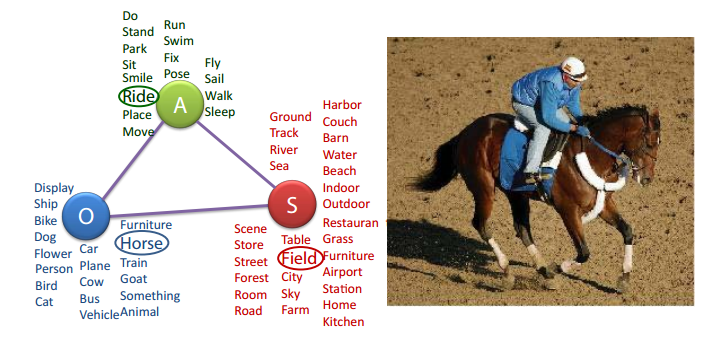
\includegraphics[scale=0.6]{./Imgs/farhadi2010every_fig2.png}
		\caption[مدل میدان تصادفی مارکف در درک صحنه]{
			طرح‌واره مدل میدان تصادفی مارکف ارائه شده در پژوهش \cite{Farhadi2010every} که شامل ۳ گره است. در این مدل، به ازای هر میدان از فضای معنا، یک گره وجود دارد و بین هر سه گره‌، به طور دو به دو، یک یال موجود است\cite{Farhadi2010every}.
		}
		\label{fig:F2010EF2}
	\end{figure}
	
	بر اساس مقادیر محاسبه شده برای ویژگی‌های بالا و با استفاده از الگوریتم ماشین بردار پشتیبان\enfootnote{Support Vector Machine (SVM)}، یک دسته‌بندی برای هر گره ارائه می‌شود که بیان‌کننده دسته ‌ویژگی‌های مربوط به مقادیر مختلف گره است. با استفاده از این دسته‌بندی، با ورود هر تصویر، می‌توان برای هر مقدار در هر گره، یک امتیاز شباهت محاسبه نمود. استفاده از الگوریتم یافتن نزدیک‌ترین همسایه‌های موجود برای هر تصویر ورودی، بر اساس امتیاز شباهت محاسبه‌شده و میانگین‌گیری روی همسایه‌های استخراج شده، معیار خوبی از تخمین مقدار هر گره، به ازای هر تصویر ورودی ایجاد می‌کند. به این ترتیب، با ورود هر تصویر می‌توان برای هر کدام از گره‌های موجود در مدل، یک مقدار محتمل مشخص نمود. سه‌تایی شامل مقادیر محتمل بدست‌آمده در هر گره، سه‌تایی متناظر تصویر ورودی در فضای معنا را مشخص می‌کند.
	\item فاکتورِ یال\\
	این فاکتور، برای مشخص کردن میزان ارتباط مقادیر مختلف دو گره با یکدیگر در تصویر ورودی مورد استفاده قرار می‌گیرند.
\end{enumerate}

%%%%%%%%%%%%%%%%%%%%%%%%%%%%%%%%%%%%%%%%%
\subsection[استفاده از مدل میدان تصادفی شرطی]{استفاده از مدل میدان تصادفی شرطی\enfootnote{Conditional Random Field (CRF)}}
مدل میدان تصادفی شرطی، یکی از پرکاربردترین مدل‌های گرافی احتمالی در زمینه درک صحنه است که پژوهش‌های متعددی از آن به عنوان مدل اصلی در درک صحنه استفاده کرده‌اند. به عنوان نمونه، در پژوهش‌های 
\cite{Lin_2013_ICCV}
و
\cite{ladicky2010and}
از مدل میدان تصادفی شرطی به منظور توصیف صحنه استفاده شده است.\\
پژوهش \cite{Lin_2013_ICCV} که توسط لین و همکارانش در سال 2013 ارائه شد، سعی در توصیف اجسام سه‌بعدی با استفاده از قطعه‌بندی تصاویر دوبعدی، هندسه سه‌بعدی و روابط بین صحنه و اجسام موجود، دارد. در این پژوهش، پس از استخراج ویژگی‌ها و اطلاعات بدست‌آمده از منابع مختلف، عمل استنتاج توسط یک مدل تصادفی شرطی انجام می‌شود که منجر به نگاشت تصویر ورودی به فضای معنایی می‌شود. همین‌طور در پژوهش \cite{ladicky2010and} که توسط لادیکی و همکارانش در سال 2010 ارائه شد، یک بستر کاری احتمالی برای استنتاج درباره نواحی مختلف تصویر، اجسام موجود و ویژگی‌های مختلف آن‌ها مانند دسته‌بندی، موقعیت مکانی و ابعاد، مبتنی بر مدل میدان تصادفی شرطی، ارائه شده است. با توجه به وسعت و تعدد فعالیت‌های انجام شده، در این بخش چزئیات یکی از روش‌های ارائه شدهر در این دسته‌بندی را مطرح نموده و از بررسی عمیق‌تر پژوهش‌های دیگر صرف‌نظر می‌نماییم.
\\
در پژوهش\cite{fidler2013sentence} که در سال 2013 توسط فیدلر و همکارانش ارائه شد،
از مدل میدان تصادفی شرطی برای توصیف صحنه و اجسام موجود در آن استفاده شده است. میدان‌های تصادفی در این مدل، شامل متغیرهای زیر هستند:
\begin{enumerate}
	\item  متغیرهای تصادفی بیان‌کننده برچسب دسته متناظر قطعات مختلف هر تصویر به شیوه سلسله مراتبی دارای دو سطح
	\item متغیرهای تصادفی باینری بیان‌کننده صحت دسته‌ تشخیص داده‌شده برای هر جسم
\end{enumerate}

شکل
\ref{fig:F2013SF1}
طرح‌واره مدل سلسله‌مراتبی ارائه شده در پژوهش \cite{fidler2013sentence} را نمایش می‌دهد. همان‌طور که مشاهده می‌شود این مدل از دو سطح انتزاع، یکی برای برچسب قطعات مختلف تصویر و دیگری برای حضور یا عدم حضور هر دسته از اجسام در تصویر، تشکیل شده است.

\begin{figure}[h]
	\center
	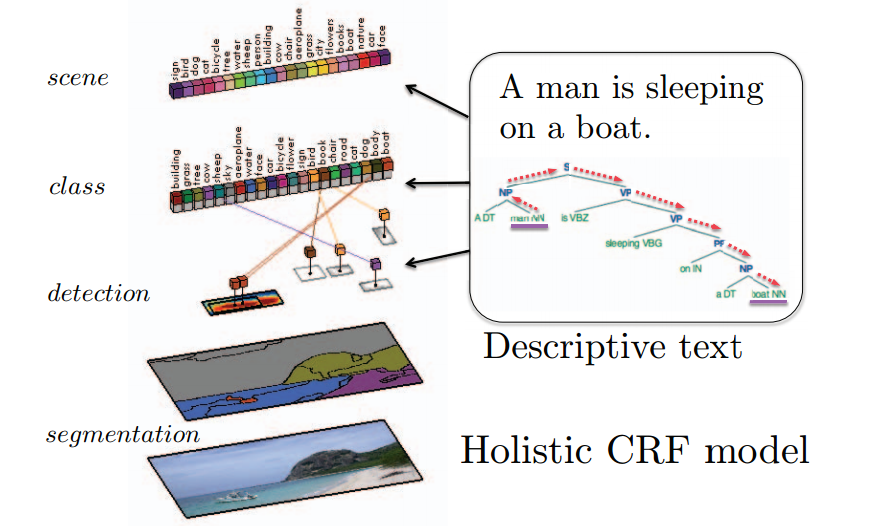
\includegraphics[scale=0.4]{./Imgs/fidler2013sentence_f1.png}
	\caption[مدل سلسله‌مراتبی میدان تصادفی شرطی در درک صحنه]{طرح‌واره مدل سلسله مراتبی مبتنی بر میدان تصادفی شرطی که بر اساس اطلاعات بصری و اطلاعات جملات توصیف‌کننده شرح محتمل تصویر را تولید می‌نماید\cite{fidler2013sentence}.}
	\label{fig:F2013SF1}
\end{figure}

دو دسته متغیر تصادفی مختلف، که هر یک نماینده متغیرهای تصادفی موجود در یکی از این سطوح انتزاع هستند، تعریف شده‌اند؛ 
متغیرهای تصادفی
 $X_i \in \{1, \cdots,C\}$ 
بیان‌کننده دسته قطعه $i$ام از سطح پایین سلسله مراتب و متغیرهای تصادفی
 $Y_j \in \{1, \cdots,C\}$ 
 بیان‌کننده دسته قطعه $j$ام از سطح بالای سلسله مراتب.
به علاوه، دو دسته متغیر تصادفی دیگر به نام‌های $b_l$ و $z_k$ به ترتیب برای نمایش حضور یا عدم حضور یک تشخیص کاندید\enfootnote{Candidate Detection} و حضور یا عدم حضور جسم با دسته $k$ در تصویر، تعریف شده‌اند. با توجه به متغیرهای تعریف شده، مدل کلی میدان تصادفی شرطی را می‌توان معادل رابطه\eqref{eq:crffidler} تعریف کرد. در این رابطه $\Psi_\alpha^{type}(a_\alpha)$ نماینده تابع پتانسیل تعریف شده روی متغیرهای مختلف است. با این تعریف، یافتن تخمین احتمال بیشینه پسین\enfootnote{MAP Estimation}، منجر به یافتن پاسخ مورد نظر می‌شود.
در ادامه، توابع پتانسیل مختلف که در این پژوهش تعریف شده‌اند، ارائه خواهد شد. لازم به ذکر است در تمام این موارد، برای سهولت، توابع پتانسیل به شکل لگاریتمی تعریف شده‌اند.
\begin{equation}
P(X,Y,b,z) = \frac{1}{Z} \mathlarger{\mathlarger{\Pi}}_{type} \mathlarger{\mathlarger{\Pi}}_\alpha \Psi_\alpha^{type}(a_\alpha)
\label{eq:crffidler}
\end{equation}

توابع پتانسیل مختلف تعریف شده در این پژوهش عبارتند از:

\begin{enumerate}
	\item پتانسیل قطعه‌بندی یگانی\enfootnote{Unary Segmentation Potential}\\
	پتانسیل قطعه‌بندی یگانی در هر قطعه و هر ابرقطعه\enfootnote{Supersegment} از تصویر، با استفاده از میانگین‌گیری روی امتیاز افزایش تکستون\enfootnote{Texton Boost} که در پژوهش \cite{ladicky2010graph} ارائه شده است، انجام می‌شود.
	\item انطباق بین متغیرهای دو سطح انتزاع با یک‌دیگر\\
	یک مقدار جریمه به ازای دسته‌های مخالف بین دو سطح در نظر گرفته‌ می‌شود تا در حد امکان، دسته‌های منتخب از بین سطوح مختلف، با یک‌دیگر انطباق داشته باشند. پتانسیل تعریف شده در این بخش معادل رابطه\ref{eq:phiijf} 
	تعریف می‌شود.
	\begin{equation}
	\phi_{ij}(X_i, Y_j)=
	\left\{
	\begin{array}{ll}
	- \gamma		&	X_i \neq Y_j \\
	0			&	X_i	=	Y_j
	\end{array}							
	\right.
	\label{eq:phiijf}
	\end{equation}
	در رابطه\ref{eq:phiijf}، پارامتر $\gamma$ در فرآیند یادگیری که منجر به بهینه‌سازی پارامترهای مختلف مدل می‌شود، به‌دست می‌آید.
	\item پتانسیل انطباق تصویر و دسته جسم\\
	برای اندازه‌گیری میزان انطباق هر کدام از دسته‌های موجود برای اجسام با تصویر ورودی، از معیار انطباق ارائه شده در پژوهش\cite{felzenszwalb2010object}
	توسط فلزنسوالب که به روش دی‌پی‌ام\enfootnote{DPM} مشهور است، استفاده شده است. برای کاهش تعداد پارامترها و افزایش کارایی مدل استفاده شده، برای هر تصویر حداکثر ۳ دسته جسم، به عنوان دسته‌های منتخب کاندید، در نظر گرفته می‌شوند.
\end{enumerate}


%%%%%%%%%%%%%%%%%%%%%%%%%%%%%%%%%%%%%%%%%
\subsection{استفاده از سایر مدل‌های گرافی احتمالی}
در بین پژوهش‌های موجود در زمینه درک صحنه با استفاده از روش‌های  گرافی احتمالی، علاوه بر مدل‌های استاندارد، از مدل‌های مولد دیگر در پژوهش‌های متعددی استفاده شده است. در ادامه این بخش، به بررسی چند‌ نمونه از این مدل‌ها خواهیم پرداخت.

\begin{enumerate}
	\item دسته‌بندی تصاویر بر اساس صحنه و اجسام موجود به طور توام\cite{li2007and}
	
	مدل استفاده شده در این پژوهش، از تصاویر در سطح صحنه و سطح اجسام استفاده کرده و با یکپارچه‌سازی و تجمیع اطلاعات موجود در این دو سطح، اقدام به دسته‌بندی تصویر می‌نماید. شکل\ref{fig:l2007af1} 
	مدل استفاده شده در این پژوهش را به منظور یکپارچه‌سازی و تجمیع اطلاعات حاصل از تحلیل صحنه و تشخیص اجسام موجود در آن، ارائه می‌دهد.
	
	
	\begin{figure}[h]
		\center
		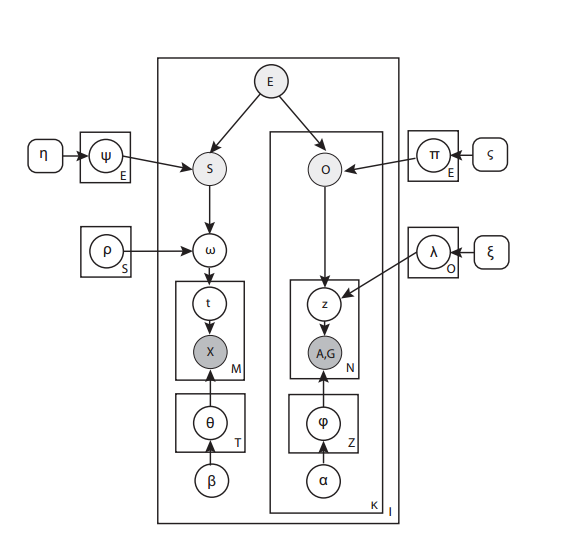
\includegraphics[scale=0.5]{./Imgs/li2007and_model.png}
		\caption[مدل گرافی احتمالی مورد استفاده در پژوهش\cite{li2007and}]{مدل استفاده شده به منظور تجمیع اطلاعات صحنه و اجسام موجود در آن به منظور دسته‌بندی تصاویر\cite{li2007and}}
		\label{fig:l2007af1}
	\end{figure}
	
	یکی از اهدافی که در این پژوهش دنبال می‌شود، برچسب‌گذاری معنایی\enfootnote{Semantic Labelling} تمام پیکسل‌های موجود در تصویر است. به همین منظور، تمام تصاویر مورد استفاده، به نواحی $10 * 10$ تقسیم شده و مورد استفاده قرار می‌گیرند. برای بررسی بهتر مدل، ابتدا متغیرهای تصادفی مورد استفاده را تعریف کرده و سپس به بررسی روند یادگیری و استنتاج مدل می‌پردازیم.
	\\
	متغیر تصادفی $X$ که حاوی اطلاعاتی مبتنی بر حضور یا عدم حضور دسته‌های مختلف صحنه است، در بخش تشخیص صحنه به‌کار می‌رود. اطلاعات این متغیر با استفاده از توصیف‌کننده سیفت\enfootnote{SIFT Descriptor} و به ازای هر ناحیه از تصویر، به‌دست می‌آید. برای بخش تشخیص اجسام موجود در صحنه، از دو منبع اطلاعاتی مختلف استفاده می‌شود. اطلاعات مربوط به حضور یا عدم حضور دسته‌های مختلف اجسام در متغیر تصادفی $A$ و اطلاعات مربوط به شکل کلی آن‌ها در متغیر تصادفی $G$ نمایش داده‌ می‌شود.
	\\
	هر گره از مدل ارائه شده، نماینده یک متغیر تصادفی است. گره‌هایی که با رنگ تیره مشخص شده‌اند، نماینده متغیرهایی هستند که در فرایند آموزش دیده می‌شوند و بقیه متغیرها، متغیرهای مخفی\enfootnote{Latent} هستند. گره‌های خاکستری روشن‌تر، متغیرهایی هستند که فقط در فرایند آموزش دیده‌ می‌شوند در حالی‌که متغیرهای تیره‌تر در هر دو فرایند آموزش و آزمون مشاهده می‌شوند.
	\\
	متغیر تصادفی $E$، نماینده یک دسته‌ از رخداد
	\enfootnote{Event}
	های ممکن است. توزیع احتمال اولیه این متغیر  تصادفی، یک توزیع یکنواخت فرض شده است که به هر تصویر ورودی، بر اساس همین توزیع، یک مقدار خاص از این متغیر تصادفی اختصاص داده می‌شود. با دانستن دسته رخداد موجود در تصویر، یک تصویر صحنه\enfootnote{Scene Image} متناظر با تصویر ورودی تولید می‌شود. با فرض وجود $S$ دسته صحنه مختلف در مجموعه‌داده، به هر تصویر، تنها یک دسته صحنه اختصاص داده می‌شود. روند اختصاص دسته صحنه به تصویر مطابق زیر است:
	\begin{itemize}
		\item[*]
		ابتدا یک دسته اولیه مطابق با توزیع احتمال شرطی 
		$P(S|E, \psi)$
		به تصویر اختصاص داده می‌شود. $\psi$ یک پارامتر چندجمله‌ای
		\enfootnote{Multinomial}
		حاکم بر توزیع احتمالاتی $S$ به شرط داشتن $E$ است. به علاوه، $\psi$ یک ماتریس به ابعاد $E * S$ و پارامتر $\eta$ یک بردار $S$ بعدی در نقش مقدار اولیه دیریکله
		\enfootnote{Dirichlet prior}
		برای پارمتر $\psi$ است.
		\item[*]
		در قدم بعدی با داشتن مقدار $S$، پارامترهای $\omega$ را بر اساس احتمال 
		$P(\omega|S, \rho)$
		تولید می‌کنیم. از آن‌جا که $\omega$ پارامتر چندجمله‌ای گره‌های مخفی $t$ هستند، باید مجموع همه آن‌ها برابر با یک باشد. به علاوه، $\rho$ یک ماتریس به ابعاد $S * T$ و مقدار اولیه دیریکله برای پارامتر $\omega$ است که در آن $T$ تعداد کل $t$ها است.
		\item[*] 
		برای تولید هر یک از $M$ ناحیه تصویر (مقادیر متغیر تصادفی $X$) به شکل زیر عملی می‌کنیم:
		\begin{itemize}
			\item[-]
			یک مقدار $t$ از توزیع احتمال $Mult(\omega)$ تولید می‌شود که مشخص‌کننده موضوعی\enfootnote{Topic} است که این ناحیه از تصویر مطابق با آن تولید شده است.
			\item[-]
			متغیر تصادفی $X$ از توزیع احتمالی 
			$P(X|t,\theta)$ تولید می‌شود.
			$\theta$ یک ماتریس به ابعاد
			$T * V_s$ است که در آن
			$V_s$ تعداد کلمات موجود در پایگاه داده مربوط به صحنه $s$  است.
			به علاوه، $\theta$ یک پارامتر چندجمله‌ای برای $X$ است و $\beta$ مقدار اولیه دیریکله برای $\theta$.
		\end{itemize}
	\end{itemize}
	
	همانند فرایندی که طی آن، تصویر صحنه به تصویر ورودی اختصاص داده می‌شود، فرایندی وجود دارد که طی آن تصویر اجسام\enfootnote{Object Image} به تصویر ورودی اختصاص داده می‌شود. بر خلاف صحنه، هر تصویر می‌تواند بیش از یک جسم داشته باشد. تعداد کل اجسام موجود در یک تصویر را با $K$ و تعداد کل دسته‌های موجود برای اجسام در مجموعه‌داده را با $O$ نمایش می‌دهیم. فرایند زیر برای هر یک از $K$ جسم موجود در تصویر اجرا می‌شود:
	
	\begin{itemize}
		\item[*]
		ابتدا یک دسته جسم با توزیع احتمالی  
		$P(O|E, \pi)$
		به تصویر اختصاص داده می‌شود که در آن، $\pi$ یک ماتریس به ابعاد $E * O$ و $\zeta$ یک بردار به طول $O$ و مقدار اولیه دیریکله پارامتر $\pi$ است.
		\item[*]
		سپس با داشتن $O$ می‌توان تمام نواحی $A$ و $G$ مرتبط با دسته جسم را تولید نمود. فرایند تولید این نواحی به شکل زیر است:
		\begin{itemize}
			\item[-]
			متغیر تصادفی مخفی $z$ که مشخص کننده موضوع است، از توزیع احتمالی $Mutl(\lambda,|O)$ تولید می‌شود. متغیر $\lambda$ یک ماتریس به ابعاد $O * Z$ است که در آن  $Z$ تعداد کل مقادیر مختلف متغیر $z$ است. به علاوه $\xi$ مقدار اولیه دیریکله برای پارامتر $\lambda$ است.
			\item[-]
			نواحی مطلوب از توزیع احتمال $P(A,G|t, \phi)$ تولید می‌شوند که در آن، $\phi$ یک ماتریس به ابعاد $Z * V_o$ است. $V_o$ تعداد کل کلمات موجود در مجموعه‌داده، به ازای نواحی $A$ و $G$ است. پارامتر $\alpha$ مقدار اولیه دیریکله برای پارامتر $\phi$
			است. 	
		\end{itemize}
	\end{itemize}
	
	با توجه به متغیرهای تصادفی توضیح داده شده در بالا، توزیع احتمالی توام کل سیستم را می‌توان مطابق با رابطه 
	\ref{eq:liJP}
	تعریف کرد.
	
	\begin{equation}
	\label{eq:liJP}\begin{split}
	P(E,S,O,X,A,G,t,z,\omega |\rho ,\phi ,\lambda ,\psi ,\pi \theta) &= P(E)\cdot P(S|E,\psi)\cdot P(\omega|S,\rho) \\ 
	&\cdot \mathlarger{\mathlarger{\Pi}}_{m=1}^M P(X_m|t_m,\theta)\cdot P(t_m|\omega) \\
	&\cdot \mathlarger{\mathlarger{\Pi}}_{k=1}^K P(O_k|E,\pi)\\
	&\cdot \mathlarger{\mathlarger{\Pi}}_{n=1}^N P(A_n,G_n|z_n,\phi)\cdot P(z_n|\lambda,O_k)
	\end{split}
	\end{equation}
	
	به علاوه، با توجه به توضیحات ارائه شده در بالا، هر کدام از عبارات موجود در رابطه \ref{eq:liJP} را می‌توان با عبارات معادل آن‌ها که در روابط
	\ref{eq:liSF}
	تا
	\ref{eq:liSL}
	آمده، جایگزین نمود.
	
	\begin{align}
	&P(S|E,\psi) = Mult(S|E,\psi)
	\label{eq:liSF}
	\\
	&P(\omega|S,\rho) = Dir(\omega|\rho_{j.}), S = j
	\\
	&P(t_m|\omega) = Mult(t_m|\omega)
	\\
	&P(X_m|t_m,\theta) = P(X_m|\theta_{j.}), t_m = j
	\\
	&P(O_k|E,\pi) = Mult(O_k|E,\pi)
	\\
	&P(z_n|\lambda,O_k) = Mult(z_n|\lambda,O_k)
	\\
	&P(A_n,G_n|z_n,\phi) = P(A_n,G_n|\phi_{j.}), z_n = j
	\label{eq:liSL}
	\end{align}
	
	درک صحنه در این پژوهش، محدود به استخراج سه دسته اطلاعات زیر از تصویر است:
	
	\begin{enumerate}
		\item رخدادی که در تصویر به نمایش گذاشته شده است.
		\item صحنه‌ای که تصویر در آن ایجاد شده است.
		\item اجسامی که در تصویر حضور دارند.
	\end{enumerate}
	
	با توجه به این محدودیت و با در نظر گرفتن مدل ارائه شده، استفاده از تخمین بیشینه احتمال\enfootnote{Maximum Likelihood}، می‌تواند برای استخراج اطلاعات مطلوب مفید باشد. از همین رو، تخمین بیشینه احتمال، در سه سطح مختلف (هر سطح برای یک دسته از اطلاعات مطلوب) اعمال می‌شود. در سطح اجسام، احتمال رخداد تصویر ورودی به شرط اجسام موجود مطابق با رابطه 
	\ref{eq:liPIO}، احتمال رخداد تصویر ورودی به شرط صحنه، مطابق با رابطه 
	\ref{eq:liPIS}
	و احتمال رخداد تصویر ورودی به شرط دسته رخداد به نمایش‌گذاشته شده در تصویر، مطابق با رابطه 
	\ref{eq:liPIE}
	محاسبه می‌شوند.
	\begin{align}
	&P(I|O) = \ML{\Pi}_{n=1}^N \ML{\Sigma}_j P(A_n,G_n|z_j,O) P(z_j|O)
	\label{eq:liPIO}
	\\
	&P(I|S,\rho,\theta) = \int P(\omega|\rho,S)(\ML{\Pi}_{m=1}^M \ML{\Sigma}_{t_m} P(t_m|\omega) P(X_m|t_m, \theta) ) d\omega
	\label{eq:liPIS}
	\\
	&P(I|E) \propto \ML{\Sigma}_j P(I|O_j) P(O_j|E) P(I|S) P(S|E)
	\label{eq:liPIE}
	\end{align}
	
	فرایند یادگیری این مدل، شامل یافتن بهترین مقادیر برای پارامترهای 
	$\{\psi,\rho,\pi,\lambda,\theta,\beta\}$
	است.
	این فرایند برای سه پارامتر 
	$\{\psi,\rho,\theta\}$ 
	با استفاده از روش انتقال پیام متغیر\enfootnote{Variational Message Passing} و برای سه پارامتر
	$\{\pi,\lambda,\beta\}$
	با استفاده از نمونه‌برداری گیبس\enfootnote{Gibbs Sampling} انجام می‌شود.
	\\
	آزمایشات انجام شده در این پژوهش، بر روی یک مجموعه‌داده شامل تصاویر از ۸ دسته ورزشی مختلف که در هر دسته، بین 137 تا 250 تصویر مختلف وجود دارد، انجام شده‌اند. از جمله چالش‌های موجود در این مجموعه‌داده می‌توان به وجود زمینه‌های متنوع و پیچیده در تصاویر، تنوع دسته‌های مختلف اجسام موجود، تنوع اندازه اجسام موجود از یک دسته، تنوع حالت اجسام، تنوع تعداد نمونه‌های یک جسم در یک تصویر و کوچک بودن بیش از اندازه ابعاد اجسام در تصویر اشاره کرد. شکل
	\ref{fig:lid}
	نمونه‌ای از تصاویر موجود در این مجموعه‌داده را نمایش می‌دهد.
	
	\begin{figure}[h]
		\center
		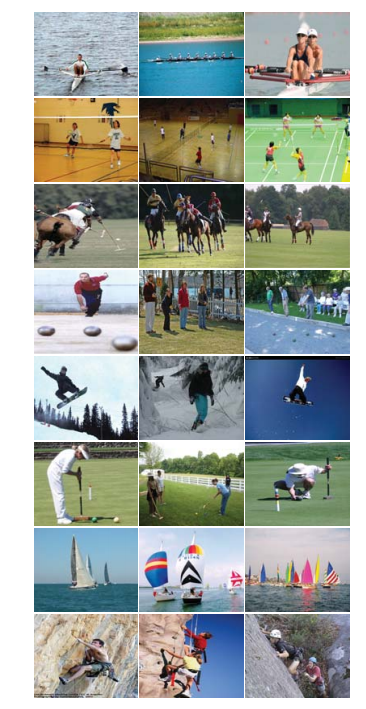
\includegraphics[scale=0.6]{./Imgs/li2007and_dataset.png}
		\caption{نمونه تصاویر موجود در مجموعه‌داده مورد استفاده \cite{li2007and}}
		\label{fig:lid}
	\end{figure}
	
	استفاده از مدل کامل ارائه شده در این پژوهش، منجر به تشخیص صحیح 73.4\% از تصاویر شده است. شکل
	\ref{fig:liCM}
	ماتریس درهم‌ریختگی
	\enfootnote{Confusion Matrix}
	مربوط به این مدل را نمایش می‌دهد. همان‌طور که در این ماتریس مشخص است، کمترین نرخ تشخیص در بین دسته‌های ورزشی موجود در این مدل، 52\% و بیشترین نرخ تشخیص 92\% است.
	
	\begin{figure}[h]
		\center
		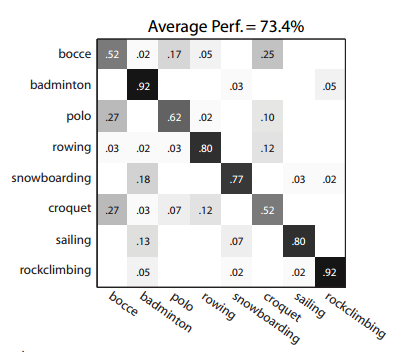
\includegraphics[scale=0.6]{./Imgs/li2007and_confmat.png}
		\caption[ماتریس درهم‌ریختگی مدل کامل ارائه شده در \cite{li2007and}]{ماتریس درهم‌ریختگی مدل کامل ارائه شده برای مجموعه‌داده شامل ۸ دسته تصویر ورزشی. \cite{li2007and}}
		\label{fig:liCM}
	\end{figure}
	
	بسته به میزان استفاده از اطلاعات مختلف استخراج شده برای استنتاج، مدل‌های مختلفی به‌وجود می‌آیند که در شکل
	\ref{fig:liCMP}
	نتایج عملکرد هریک از این مدل‌ها با مدل‌های دیگر مقایسه شده است.
	همان‌طور که در شکل \ref{fig:liCMP}
	مشخص است، بهترین کارایی مربوط به مدل کامل است. در صورتی‌که در مدل، فقط از اطلاعات مربوط به صحنه استفاده شود، نتایج بدست‌آمده اگرچه با نتایج مدل کامل قابل مقایسه نیست، از نتایج مدل مبتنی بر اطلاعات جسم بهتر است.
	
	\begin{figure}[h]
		\center
		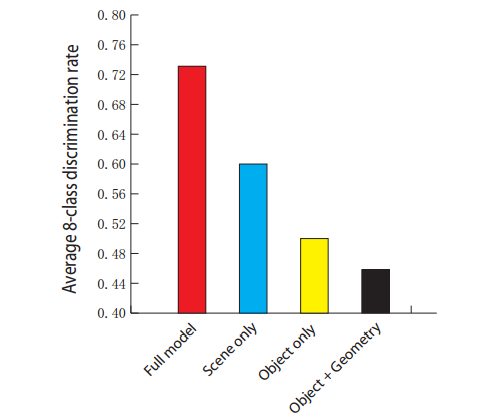
\includegraphics[scale=0.4]{./Imgs/li2007and_compar.png}
		\caption[نتیجه مقایسه مدل‌های مختلف در \cite{li2007and}]{نتیجه مقایسه مدل‌های مختلف به‌وجود آمده بسته به سطح اطلاعات مورد استفاده برای استنتاج. \cite{li2007and}}
		\label{fig:liCMP}
	\end{figure}
	
	شکل
	\ref{fig:liR}
	نتایج نهایی به‌دست آمده از مدل را نمایش می‌دهد. در این شکل، تصاویر موجود در هر سطر نماینده تصاویر موجود در یکی از دسته‌های ورزشی هستند. ستون اول برچسب به‌دست آمده از رخداد موجود در تصویر، ستون دوم برچسب‌های تشخیص داده شده مربوط به اجسام موجود، ستون سوم برچسب اختصاص داده‌شده مربوط به دسته صحنه و ستون چهارم توزیع مرتب شده اجسام به شرط رخداد را به نمایش می‌گذارند. در نمودارهای موجود در ستون چهارم، محور افقی شامل نام اجسام و محور عمودی مقدار توزیع را نمایش می‌دهد.
	
	\begin{figure}
		\center
		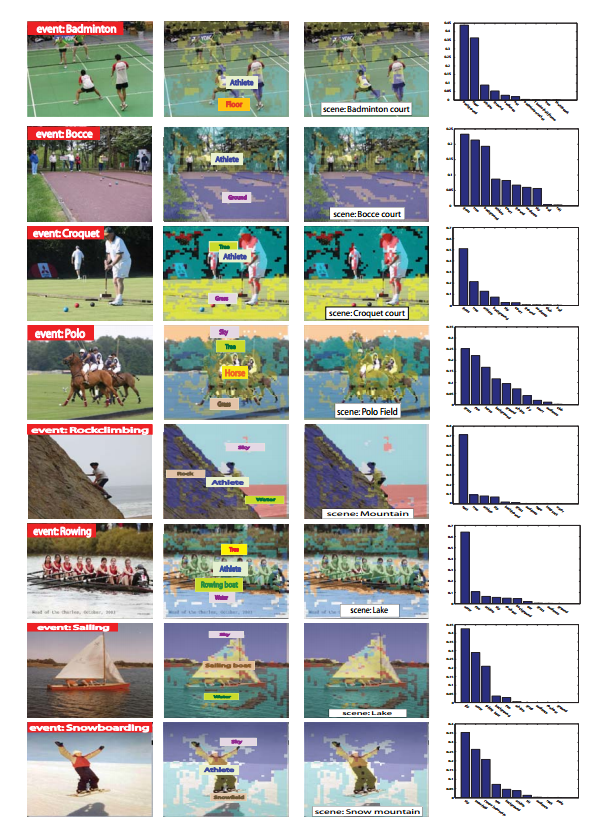
\includegraphics[height=0.9\textheight]{./Imgs/li2007and_res1.png}
		\caption{نتایج نهایی به‌دست آمده از مدل بر روی تصاویر. \cite{li2007and}}
		\label{fig:liR}
	\end{figure}
	
	
	
	%%%%%%%%%%%%%%%%%%%%%%%%%%%%%%%%%%%%%%%%%%%%%%%%%%%%
	%\item حاشیه‌نویسی تصویر\enfootnote{Image Annotation} با استفاده از قطعه‌بندی و دسته‌بندی صحنه و اجسام موجود\cite{li2009towards}
	%
	%
	%
	%
	%
	%\item درک صحنه بر اساس نواحی مختلف تصویر، اجسام موجود و روابط سه‌بعدی بین ‌آن‌ها\cite{gould2009decomposing}
\end{enumerate}

%%%%%%%%%%%%%%%%%%%%%%%%%%%%%%%%%%%%%%%%%
\section{روش‌های مبتنی بر شبکه‌های عصبی کانولوشنی عمیق}

علاوه بر فعالیت‌هایی که در زمینه تولید خودکار شرح بر تصاویر با استفاده از مدل‌های گرافی احتمالی انجام شده‌اند، تعداد زیادی از پژوهش‌گران تلاش می‌کنند تا با استفاده از روش‌‌های مبتنی بر شبکه‌های عصبی با این چالش روبرو شوند. در این بخش تعدادی از پژوهش‌هایی را که با استفاده از شبکه‌های عصبی سعی در درک صحنه‌های موجود در تصاویر دارند را مورد بررسی قرار می‌دهیم. 
\\
یکی از مهم‌ترین بخش‌هایی که به نحوی در پژوهش‌های قبلی انجام می‌شد، اختصاص یک معنا به قطعه‌های مختلف یک تصویر است. این چالش، در پژوهش‌های مرتبط با تولید خودکار شرح بر تصاویر که با استفاده از روش‌های مبتنی بر شبکه‌های عصبی به دنبال حل مشکل هستند نیز مطرح است. در ابتدا به بررسی یکی از روش‌های اختصاص معنا به هر قطعه ازتصویر می‌پردازیم.

\subsection[اختصاص معنا به قطعه‌های مختلف تصویر]{اختصاص معنا به قطعه‌های مختلف تصویر\cite{Girshick_2014_CVPR}}
در پژوهش 
\cite{Girshick_2014_CVPR}
که توسط گرشیک و همکارانش در سال 2014 انجام شده،
روشی ارائه شده است که با استفاده از یک شبکه عصبی کانولوشنی عمیق، علاوه بر این که می‌تواند یک تصویر را به شکل پایین به بالا، در قالب نواحی سلسله‌مراتبی قطعه‌بندی کند، قادر به استفاده به عنوان یک شبکه از پیش آموزش  دیده‌شده در پژوهش‌های مرتبط دیگر باشد.
\\
فرایند تشخیص اجسام در این پژوهش از سه بخش اصلی تشکیل شده است:
\begin{enumerate}
	\item
	طرح پیشنهاداتی برای نواحی به طور مستقل از دسته‌بندی\enfootnote{Category-independent region proposals}
	\item 
	یک شبکه عصبی عمیق کانولوشنی که وظیفه استخراج ویژگی برای هر ناحیه را بر عهده دارد (طول بردار ويژگی استخراج شده برای تمام نواحی یکسان است).
	\item
	مجموعه‌ای از ماشین‌های بردار پشتیبان خطی مخصوص هر دسته
\end{enumerate}
در ادامه به بررسی نحوه پیشنهاد نواحی و شبکه عصبی کانولوشنی عمیق مورد استفاده در ای پژوهش می‌پردازیم.

\begin{enumerate}
	\item طرح پیشنهاد نواحی\\
	روش‌های مختلفی برای پیشنهاد نواحی ارائه شده‌اند که در اینجا از روشی موسوم به جستجوی انتخابی\enfootnote{Selective Search} استفاده می‌شود. نسخه‌های مختلفی از این روش ارائه شده است. نسخه ارائه شده در پژوهش
	\cite{uijlings2013selective}،
	یکی از سریع‌ترین نسخه‌های ارائه شده است که در این بخش از همین روش استفاده می‌شود.
	\\
	در پژوهش 
	\cite{uijlings2013selective}
	دو ویژگی‌ مطرح شده است که یک جستجوی انتخابی برای ارائه نواحی معنایی تصویر باید آن‌ها را داشته باشد. ویژگی اول این است که اجسام موجود در فضا می‌توانند در هر اندازه‌ای باشند و در نتیجه نواحی ارائه شده باید بتوانند ابعاد مختلف داشته باشند. این ویژگی عموما با روش‌های سلسله‌مراتبی قابل دست‌یابی است. ویژگی دوم این است که نواحی مختلف باید براساس  ویژگی‌های مختلفی تولید شوند. در صورتی‌که یک ویژگی مثل رنگ، بافت، روشنایی یا مواردی از این دست، به عنوان تنها ویژگی برای تشخیص نواحی به کار گرفته شود، الگوریتم قادر به ارائه نواحی مناسب در شرایط مختلف نخواهد بود. بنابراین ترکیب چند معیار و ویژگی باید برای تشخیص نواحی مورد استفاده قرار بگیرد. 
	\\
	برای دست‌یابی به ویژگی اول، ابتدا نواحی اولیه کوچکی روی تصویر ایجاد می‌شود. سپس با اتخاذ یک روش حریصانه و تعریف یک معیار شباهت بین نواحی همسایه، ناحیه‌هایی که شباهت زیادی با یک‌دیگر دارند و همسایه هستند، با هم ترکیب شده و یک ناحیه بزرگ‌تر ساخته می‌شود. به این ترتیب یک روش سلسله‌مراتبی برای ساخت نواحی با ابعاد مختلف به‌دست ‌می‌آید.برای دست‌یابی به ویژگی دوم، از فضاهای رنگی مختلف، معیارهای شباهت مختلف و نواحی اولیه متفاوت و ترکیب پاسخ این ویژگی‌ها با هم برای ارائه نواحی و ترکیب نواحی کوچک‌تر استفاده می‌شود.
	
	\item شبکه عصبی کانولوشنی عمیق (استخراج ویژگی‌ها)\\
	در این بخش از یک شبکه عصبی کانولوشنی عمیق از پیش‌آموزش‌دیده‌ برای استخراج ویژگی ‌از هر ناحیه ارائه شده در قسمت قبل، استفاده می‌شود. بردار ویژگی استخراج شده برای هر ناحیه یک بردار شامل 4096 مولفه است که خروجی شبکه کریشفسکی\enfootnote{Krizhevsky}
	آزمایش شده در چالش دسته‌بندی اجسام مسابقه  \lr{ImageNet} است. اطلاعات دقیق درباره این شبکه عصبی در پژوهش 
	\cite{krizhevsky2012imagenet}
	در دسترس است.
	
\end{enumerate}

شبکه عصبی کانولوشنی عمیق ارائه شده در این پژوهش با استفاده از یک مجموعه‌داده\enfootnote{ILSVRC 2012} آموزش دیده شده است. از این شبکه عصبی که تحت عنوان \lr{RCNN}\enfootnote{Regional Convolutional Neural Network} شناخته می‌شود می‌توان به عنوان یک شبکه از پیش‌آموزش‌دیده استفاده کرد.

\subsection[ناحیه‌بندی عمیق تصاویر به منظور نگاشت دوطرفه جملات و تصاویر]{ناحیه‌بندی عمیق تصاویر به منظور نگاشت دوطرفه جملات و تصاویر\cite{karpathy2014deep}}

مدل ارائه شده در این پژوهش، مدلی است که قادر به نگاشت دوطرفه تصاویر و جملات به یک‌دیگر است. شکل
\ref{fig:k2014DM} 
طرح‌واره‌ای از این مدل را نمایش می‌دهد. ورودی مدل در سمت چپ، تصاویر و در سمت راست، جملات هستند. در این مدل، ابتدا تصاویر ورودی با استفاده از یک شبکه عصبی 
\lr{RCNN}
 تبدیل به نواحی مختلف شده و برای هر ناحیه یک بردار ویژگی 4096 بعدی استخراج می‌شود. سپس با اعمال روش خاصی روی جملات ورودی از سمت راست (که در بخش تولید جملات زبان طبیعی به بررسی آن خواهیم پرداخت) قطعات مختلف موجود در جملات نیز استخراج شده و بین هر قطعه از جمله با تمام نواحی استخراج شده از تصویر یک معیار شباهت محاسبه می‌شود و شبیه‌ترین قطعه جمله با ناحیه مربوط به خود در تصویر، جفت می‌شوند.

\begin{figure}[h]
	\center
	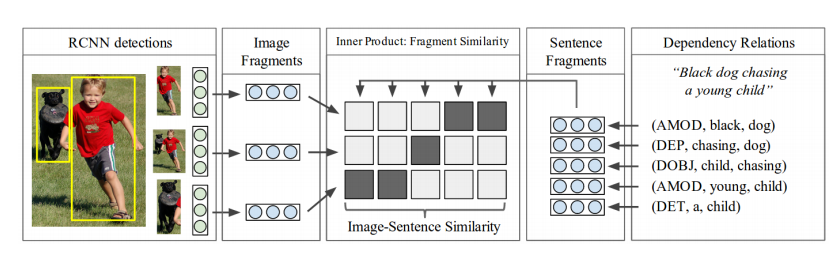
\includegraphics[scale=0.5]{./Imgs/karpathy2014deep_model.png}
	\caption[طرح‌واره عملکرد روش \lr{RCNN}]{مدل استفاده شده برای نگاشت دو‌طرفه تصاویر و جملات به یک‌دیگر با استفاده از شکبه‌ عصبی عمیق کانولوشنی.\cite{karpathy2014deep}}
	\label{fig:k2014DM}
\end{figure}

در این پژوهش پس از ناحیه‌بندی تصویر توسط شبکه \lr{RCNN}، برای هر تصویر ۱۹ ناحیه استخراج می‌شود. این ۱۹ ناحیه در کنار تصویر اصلی، یک مجموعه شامل ۲۰ تصویر ایجاد می‌کنند که در پردازش‌های بعدی مورد استفاده قرار خواهند گرفت. در این مرحله باید تمام تصاویر موجود را با استفاده از یک نگاشت به فضای برداری ویژگی‌ها تبدیل نمود. برای این کار از رابطه\ref{eq:k2014ISV}
استفاده می‌شود. در این رابطه، $I_b$ مجموعه تمام پیکسل‌های موجود در ناحیه $b$،
$RCNN_{\theta_c}$
شبکه عصبی آموزش‌دیده است که در آن $\theta_c$ مجموعه پارامترهای بهینه موجود در شبکه است. بردار حاصل $\nu_i$ برای تصویر $i$ام، بردار نگاشت تصویر به فضای معنایی خواهد بود که محاسبه مقادیر آن مبتنی بر پیشنهاد نواحی معنایی مختلف و محاسبه ويژگی‌های مختلف روی هر ناحیه است.

\begin{equation}
\nu = W_m[RCNN_{\theta_c}(I_b)] + b_m
\label{eq:k2014ISV}
\end{equation}

از طرفی با در نظر گرفتن بردار $s_j$ به عنوان بردار حاصل از نگاشت جمله $j$ام به فضای معنایی و در نظر گرفتن ضرب داخلی به عنوان شباهت، $\nu_i^T \cdot s_j$
معیار شباهت بین یک تصویر و یک جمله را تعریف می‌کند.
با توجه به توضیحات ارائه شده، می‌توان تابع هدف را برای شبکه کلی معادل سیستم ارائه داد. دو هدف اصلی در این شبکه قابل تعریف است:
\begin{enumerate}
	\item رتبه‌بندی سراسری\\
	تصاویر و جملاتی که در فرایند محاسبات شبکه عصبی بیشترین شباهت را با یک‌دیگر دارند باید در واقعیت هم بیشترین شباهت و ارتباط را داشته باشند.
	\item هم‌ترازسازی ناحیه‌ای\enfootnote{Fragment Alignment}\\
	نواحی استخراج شده تصویر و عبارات استخراج شده جملات که در محاسبات شبکه عصبی بیشترین شباهت را با یک‌دیگر دارند، باید در واقعیت هم بیشترین شباهت و ارتباط را داشته باشند.
\end{enumerate}

با توجه به مطالب گفته شده، می‌توان تابع هدف کلی را مطابق با رابطه\ref{eq:k2014Obj}
تعریف کرد.
در این رابطه، $\Theta$ مجموعه پارامترهای شبکه عصبی شامل 
$\{W_m,b_m,\theta_c,W_e,W_R\}$
است (پارامترهای $W_e$ و‌ $W_R$ مربوط به بخش تحلیل جمله هستند که در فصل مربوطه بررسی خواهند شد). $C_F$ تابع هدف هم‌ترازسازی ناحیه‌ای، $C_G$ تابع هدف سراسری، $\alpha$ و $\beta$ دو ابرپارامتر\enfootnote{Hyperparameter} (با آزمون و خطا تعیین می‌شوند) و $||\Theta||_2^2$ یک عبارت تنظیم‌کننده\enfootnote{Regularization Term} هستند.

\begin{equation}
C(\Theta) = C_F(\Theta) + \beta C_G(\Theta) + \alpha ||\Theta||_2^2
\label{eq:k2014Obj}
\end{equation}

در ادامه به تعریف هریک از اهداف بیان‌شده می‌پردازیم.

\begin{enumerate}
	\item هم‌ترازسازی ناحیه‌ای 
	
	هدف از هم‌ترازسازی ناحیه‌ای این است که اگر عبارتی از یک جمله با یک تصویر شباهت زیادی پیدا کرد، حداقل یک ناحیه از تصویر وجود داشته باشد که نمایش‌دهنده این عبارت باشد و بقیه نواحی تصویر، ارتباط کمی با این عبارت داشته باشند. به عبارت بهتر، در صورتی‌که شباهت یک عبارت از یک جمله با یک تصویر از حدی بیشتر شد، شباهت حداقل یکی از نواحی موجود در تصویر با این عبارت زیاد شده و شباهت بقیه نواحی تصویر با آن کم شود. این فرض در سه حالت، رد می‌شود. اولین حالت، حالتی است که در آن ناحیه‌ای که در واقه نمایش‌دهنده عبارت است، توسط \lr{RCNN} تشخیص داده نشده باشد. دومین حالت، حالتی است که عبارت موجود به هیچ بخشی از ویژگی‌های بصری تصویر اشاره نکند و آخرین حالت، حالتی است که عبارت توصیف‌کننده، در هیچ یک از تصاویر دیگر تکرار نشده باشد در صورتی‌که ممکن است تصاویر دیگری هم وجود داشته باشند که شامل ویژگی‌های بصری متناظر با عبارت باشند. با توجه به شرایطی که فرض در آن‌ها نقض می‌شود، می‌توان آن را یک فرض خوب تلقی کرد که در اکثر موارد عملکرد خوبی دارد.
	\\
	رابطه\ref{eq:k2014C0}
	تابع هدف هم‌ترازسازی ناحیه‌ای را تعریف‌ می‌کند. در این رابطه، $y_{ij}$ برای تصویر $i$ام و جمله $j$ام در صورتی‌که با هم در مجموعه‌داده حضور داشته باشند، +1 و در غیر این‌ صورت، -1 خواهد شد.
	
	\begin{equation}
	C_0(\Theta) = \ML{\Sigma}_i \ML{\Sigma}_j max(0 , 1 - y_{ij} \nu_i^T \cdot s_j)
	\label{eq:k2014C0}
	\end{equation}
	
	تابع $C_0$ تعریف شده، باعث می‌شود در حالاتی که تصویر و عبارت، در مجموعه‌داده، با یک‌دیگر وارد شده باشند امتیاز تابع هدف بیشتر از +1 شود و در غیر این‌صورت از -۱ کمتر شود. شکل\ref{fig:k2014dCFG}،
	دو نمونه از تصاویر و جملات موجود در مجموعه‌داده را نمایش می‌دهد. 
	$C_0$ 
	در سلول‌هایی که با رنگ قرمز مشخص شده‌اند، امتیاز را به سمت کمتر از -1 حرکت می‌دهد و در بقیه سلول‌ها به سمت بیشتر از +1.
	
	به عبارت بهتر، $C_0$ یک امتیاز برای مجموع تفاوت‌های نواحی مختلف از تصاویر با عبارات مختلف جملات است. به دلیل این‌که این معیار، باعث دیده نشدن موارد کم‌یاب می‌شود، با متغیر گرفتن پارامتر $y_{ij}$ سعی در یافتن کمترین مقدار آن می‌کنیم. رابطه 
	\ref{eq:k2014CF}
	معیار متناظر با هدف کلی هم‌ترازسازی ناحیه‌ای را بیان می‌کند.
	
	\begin{align}
	&C_F(\Theta) = min_{y_{ij}} C_0(\Theta)
	\nonumber
	\\
	&s.t. \ML{\Sigma}_{i \in p_j} \frac{y_{ij} + 1}{2} \geq 1 \land
	&y_{ij} = -1, \forall i,j ; m_\nu(i) \neq m_s(j) \land y_{ij} \in \{+1, -1\}
	\label{eq:k2014CF}
	\end{align}
	
	در این رابطه، $p_j$ مجموعه تصاویر موجود در کیسه‌ مثبت\enfootnote{Positive Bag} مربوط به عبارت $j$ام است. شایان ذکر است، تنها تصاویری که در مجموعه‌داده همراه با عبارت $j$ام مشاهده شده‌اند در کیسه‌ مثبت مربوط به این عبارت قرار می‌گیرند و بقیه تصاویر در کیسه منفی\enfootnote{Negative Bag} این عبارت قرار می‌گیرند. $m_\nu(i)$ و $m_s(j)$ به ترتیب، شماره تصویر و عبارت را در مجموعه‌داده مشخص می‌کنند. 
	
	\begin{figure}[h]
		\center
		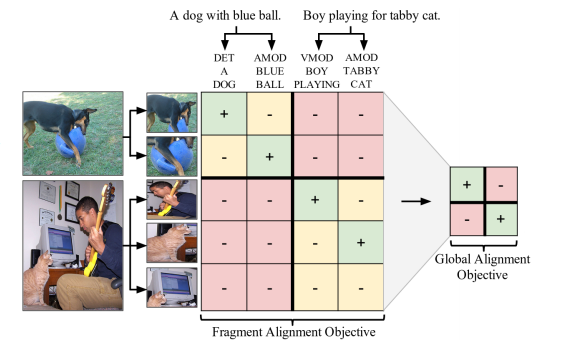
\includegraphics[scale=0.5]{./Imgs/karpathy20014deep_CFG.png}
		\caption[نتایج عملکرد اهداف تعریف‌شده در روش \lr{RCNN} برای هم‌ترازسازی تصاویر و جملات]{دو نمونه از تصاویر و جملات مرتبط با آن‌ها و نتایج  عملکرد اهداف تعریف‌شده روی آن‌ها. سطرها نمایش‌دهنده نواحی مختلف تصویر و ستون‌ها نمایش ‌دهنده قطعه‌های مختلف جملات هستند. سلول‌های قرمز رنگ حالاتی هستند که در آن‌ها $y_{ij} = -1$، سلول‌های زرد نمایش‌دهنده اعضای کیسه‌های مثبت هستند که در آن‌ها $y_{ij} = -1$ است. \cite{karpathy2014deep}}
		\label{fig:k2014dCFG}
		
	\end{figure}
	
	\item رتبه‌بندی سراسری
	
	هدف از رتبه‌بندی سراسری این است که شباهت بین یک تصویر و یک جمله، بیشینه شود اگر و تنها اگر تصویر و جمله در واقعیت نیز بیشترین شباهت را به یک‌دیگر داشته باشند. برای این منظور، ابتدا یک امتیاز شباهت بین یک تصویر و یک جمله تعریف می‌شود. این امتیاز مطابق با رابطه\ref{eq:k2014CGS}
	تعریف شده و برابر است با میانگین امتیاز شباهت دوبه‌دوی نواحی مختلف تصویر با عبارات مختلف جمله.
	
	\begin{equation}
	S_{kl} = \frac{1}{|g_k| (|g_l| + n)} \ML{\Sigma}_{i \in g_k}\ML{\Sigma}_{j\in g_l}max(0,\nu_i^T\cdot s_j)
	\label{eq:k2014CGS}
	\end{equation}
	
	از آن‌جا که برای دسته‌بندی از روش \lr{mi\_SVM} استفاده می‌شود، تمام امتیازها به صفر محدود می‌شوند. مقدار $n$ که در مخرج کسر اضافه شده است، به صورت تجربی و با آزمون و خطا به‌دست آمده که نتایج را بهبود می‌بخشد. مقدار پیشنهاد شده در پژوهش، $n = 5$ است. تابع کلی هدف سراسری مطابق با رابطه \ref{eq:k2014CG}
	تعریف می‌شود.
	
	\begin{equation}
	C_G(\Theta) = \ML{\Sigma}_k(
	\ML{\Sigma}_l max(0, S_{kl} - S{kk} + \Delta) + 
	\ML{\Sigma}_l max(0, S_{lk} - S{kk} + \Delta) 
	)
	\label{eq:k2014CG}
	\end{equation}
	
	در رابطه ارائه شده، $\Delta$ یک ابرپارامتر است که با آزمون و خطا به‌دست می‌آید. عبارت اول درون پرانتز بیان‌کننده امتیاز تصویر و عبارت دوم بیان‌کننده امتیاز جمله هستند.
\end{enumerate}


شکل\ref{fig:k2014res1}
نتایج روش پیشنهاد شده در این پژوهش را ارائه می‌دهد. همان‌طور که در شکل مشخص است، این شبکه قادر به تشخیص اجسام مختلف در تصویر و تولید یک سه‌تایی متناظر هر جسم (ناحیه معنایی) مبتنی بر جملات موجود در مجموعه‌داده مورد استفاده است.

\begin{figure}[h]
	\center
	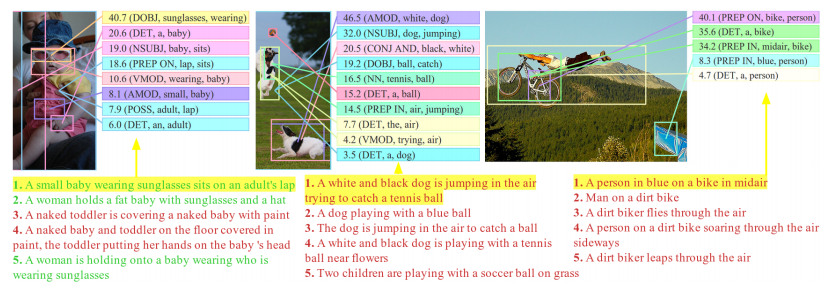
\includegraphics[scale=0.5]{./Imgs/karpathy2014deep_res1.png}
	\caption[نتایج نهایی روش \lr{RCNN}]
	{نتایج نهایی شبکه عصبی ارائه شده. برای هر ناحیه معنایی از تصویر، یک سه‌تایی مبتنی بر جملات موجود در مجموعه‌داده تولید شده است. همین‌طور 5 جمله تولید شده برای هر تصویر به ترتیب امتیاز، درج شده‌اند.\cite{karpathy2014deep}}
	\label{fig:k2014res1}
\end{figure}

به علاوه، با توجه به مدل ارائه شده و نگاشت دوطرفه موجود بین تصاویر و جملات، می‌توان با ورودی دادن یک جمله، تصاویر مربوط به آن جمله را استخراج نمود. شکل\ref{fig:k2014res2}
با ثابت در نظر گرفتن جملات، تصاویر مربوط به هر جمله را استخراج و نمایش داده است. هر سطر از این شکل، نمایش‌دهنده تصاویر استخراج شده مرتبط با جمله موجود در آن سطر است.



\begin{figure}[h]
	\center
	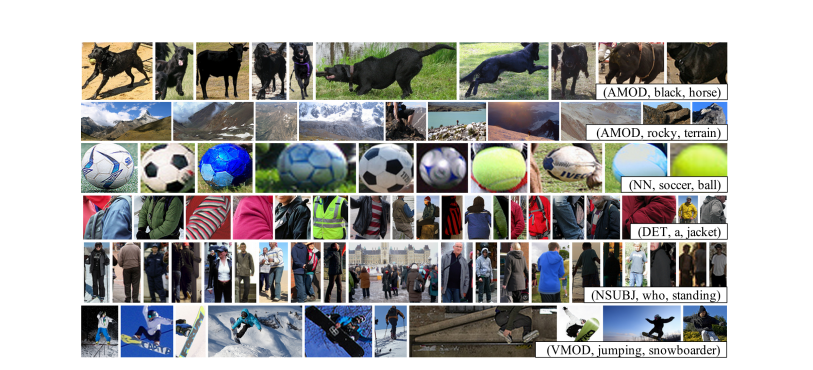
\includegraphics[scale=0.5]{./Imgs/karpathy2014deep_res2.png}
	\caption[نتایج حاصل از جستجوی جملات در روش \lr{RCNN}]{نتایج حاصل از جستجوی جملات. با ورودی دادن یک جمله، شبکه عصبی ارائه شده در این پژوهش، قادر به استخراج تصاویر مربوط به آن جمله است.\cite{karpathy2014deep}}
	\label{fig:k2014res2}
\end{figure}

روش ارائه شده در این پژوهش، به طور کامل و دقیق در پژوهش \cite{Karpathy_2015_CVPR} هم مورد استفاده قرار گرفته است، با این تفاوت که در فرایند تحلیل جمله، تغییراتی ایجاد شده است. جزئیات این روش در فصل تولید جملات زبان طبیعی مورد بررسی قرار خواهد گرفت.

\subsection{مدل دوطرفه نگاشت تصاویر و جملات مبتنی بر یادگیری عمیق}
یکی از مشکلات عمده در روش‌های مبتنی بر یادگیری عمیق، وجود حافظه مناسب برای به‌‌ خاطرسپاری رخ‌دادهای گذشته است. در شبکه‌های عصبی پیش‌رو عمیق که دارای $l$ لایه هستند، ظرفیت حداکثر حافظه موجود برای رخ‌دادهای گذشته $l-1$ است و شبکه قادر است تنها $l-1$ رخ‌داد گذشته را به‌ خاطر بسپارد. شبکه‌های عصبی بازگشتی، تا حد خوبی این مشکل را برطرف می‌نمایند. به همین دلیل، استفاده از این دسته از شبکه‌ها در بخش تولید جمله، منجر به ایجاد نتایج بهتر می‌شود. 
\\
با این حال، شبکه‌های عصبی بازگشتی نیز در مواردی که طول جمله زیاد باشد، قادر به به‌خاطرسپاری مناسب رخ‌دادهای گذشته نیستند. برای رفع این مشکل، معمولا از واحد‌های گیت در شبکه‌های عصبی حافظه کوتاه‌مدت بلند استفاده می‌شود. در پژوهش \cite{mikolov2010recurrent} که توسط خانم مایکولوف
\enfootnote{Mikolov}
در سال 2010 ارائه شده است، شبکه عصبی‌ای ارائه شده است که بدون استفاده از واحدهای گیت، قادر به حفظ رخ‌دادهای گذشته دور است. پژوهش \cite{chen2015mind} که در سال 2015 توسط آقای زیتنیک و همکارانش ارائه شده است، با استفاده از شبکه عصبی ارائه شده توسط خانم مایکولوف، مدلی دوطرفه برای نگاشت تصاویر و جملات به یک‌دیگر ارائه شده است که با داشتن تصویر قادر به تولید شرح متناظر و با داشتن شرح، قادر به بازسازی تصویر مربوطه است.
\\
در ادامه، ابتدا مدل مطرح‌شده توسط خانم مایکولوف را به طور مختصر شرح داده و سپس به بررسی مدل ارائه شده توسط آقای زیتنیک می‌پردازیم.

\subsection{مدل زبانی مبتنی بر شبکه عصبی بازگشتی}
در این قسمت به بررسی مدل زبانی ارائه شده توسط خانم مایکولوف در پژوهش \cite{mikolov2010recurrent} می‌پردازیم. مدل ارائه شده در این پژوهش، یک مدل بسیار ساده از یک شبکه عصبی بازگشتی است. در لایه ورودی شبکه، کلمات موجود در جمله به ترتیب وارد می‌شوند. برای افزایش سرعت عملیات، به جای خود کلمات از نشان\enfootnote{Token} در نظر گرفته شده برای کلمه استفاده می‌شود. برای محاسبه خروجی شبکه می‌توان از روابط \eqref{eq:4-mik1} تا \eqref{eq:4-mik5} استفاده نمود که در آن‌ها، $w(t)$ کلمه $t$ام موجود در جمله، $s(t-1)$ بردار حالت شبکه در زمان 
$t-14$
، $u_{j,i}$
وزن مربوط به اتصال ورودی واحد به بردار حالت شبکه، $v_{kj}$ بردار وزن مربوط به بردار حالت شبکه و خروجی آن و $y_k$ خروجی مرحله $k$ام مدل را نمایش می‌دهند.

\begin{align*}
	x(t) &= W(t) + s(t-1) 
	\numberthis \label{eq:4-mik1} \\
	s_j(t) &= f(\Sigma_i x_i(t)u_{ji}) 
	\numberthis \label{eq:4-mik2} \\
	y_k(t) &= g(\Sigma_j s_j(t)v_{kj}) 
	\numberthis \label{eq:4-mik3} \\
	f(z) &= \frac{1}{1 + e^{-z}} 
	\numberthis \label{eq:4-mik4} \\
	g(z_m) &= \frac{e^{z_m}}{\Sigma_k e^{z_k}}
	\numberthis \label{eq:4-mik5}
\end{align*}

\subsection{مدل دوطرفه نگاشت تصاویر و جملات با استفاده از شبکه عصبی بازگشتی}

در مدل ارائه شده در پژوهش \cite{chen2015mind}  که توسط آقای زیتنیک در سال 2015 ارائه شد، با تغییر مدل زبانی ارائه شده توسط خانم مایکولوف و تبدیل آن به یک مدل دوطرفه، روشی برای نگاشت دوطرفه تصاویر و جملات به یک‌دیگر ارائه شده است. در این بخش به بررسی این مدل و نحوه عمل‌کرد آن به طور اجمالی، خواهیم پرداخت.
\\
در این پژوهش، دو متغیر جدید به مدل زبانی مطرح شده اضافه شده‌اند. متغیر $V$ که بیان‌گر بردار ویژگی تصویر است و برای منوط کردن معنای جمله به ویژگی‌های تصویر مورد اسفاده قرار می‌گیرد و متغیر $U$ که یک متغیر مخفی است و بیان‌گر تفسیر بصری آخرین کلمه مشاهده شده یا تولید شده است.
\\
برای تولید یک مدل دوطرفه، کافیست بتوانیم احتمال رخ‌داد جمله به شرط داشتن تصویر و همین‌طور احتمال رخداد تصویر به شرط جمله را محاسبه نماییم. همین‌طور این کار را می‌توان با بخش‌هایی از تصویر و کلمات جمله انجام داد؛ به این معنی که با مدل‌کردن احتمال رخ‌داد بخش‌هایی از تصویر به شرط داشتن کلمه‌ای از جمله و همین‌طور احتمال رخ‌داد کلمه‌ای در جمله با داشتن بخشی از تصویر به طور همزمان، یک نگاشت دوطرفه بین تصاویر و جملات مرتبط با آن‌ها ایجاد نماییم.
\\
این کار را می‌توان مطابق با رابطه \eqref{eq:4-mind1} انجام داد. این رابطه، محاسبه‌کننده میزان درست‌نمایی کلمه $w_t$ و بردار ویژگی $V$ به شرط داشتن کلمات قبلی $W_{t-1}$ و تفسیر بصری هرکدام از آن‌ها $U_{t-1}$ است. 
\begin{equation}
P(w_t, V | W_{t-1} , U_{t-1}) = P(w_t | V, W_{t-1} , U_{t-1}) P(V| W_{t-1}, U_{t-1})
\label{eq:4-mind1}
\end{equation}

همان‌طور که در رابطه \eqref{eq:4-mind1} مشخص است، می‌توان این رابطه را به شکل حاصل‌ضرب دو عبارت نوشت که هریک از آن‌ها قابلیت مدل‌شدن توسط یک شبکه عصبی بازگشتی را دارند. از طرفی متغیر‌های مورد استفاده در هر دو عبارت یکسان است و فقط جهت محاسبات متفاوت است. این نکته باعث می‌شود بتوانیم از یک شبکه عصبی بازگشتی به شکل دوطرفه برای مدل‌سازی کامل رابطه درست‌نمایی توام استفاده نماییم.
\\
شکل \ref{fig:4-mind1} ساختار کلی شبکه ارائه شده در این پژوهش را نمایش می‌دهد. در این تصویر، شکل سمت چپ نمایش‌دهنده مدل به طور کامل است و شکل‌های وسط و سمت راست به ترتیب نمایش‌دهنده بخش‌هایی از مدل هستند که برای تولید جمله با داشتن تصویر و تولید تصویر با داشتن جمله مورد استفاده قرار می‌گیرند.
\\
شکل \ref{fig:4-mind1} ساختار مدل زبانی ارائه شده توسط خانم مایکولوف را نمایش می‌دهد که متغیرهای $V$ و $W$ به آن اضافه شده‌اند. اضافه کردن یک لایه $V$ به مدل زبانی، که در شکل با رنگ سفید مشخص شده است، این امکان را می‌دهد که اطلاعات مختلفی را بتوان در مدل زبانی در نظر گرفت. این اطلاعات می‌توانند اطلاعات مربوط به نقش کلمات در جمله، مدل عنوان\enfootnote{Topic Model} و مواردی از این دست باشد. در این پژوهش از بردار ویژگی تصویر که مشخص‌کننده معنای تصویر است برای این قسمت استفاده شده است. این کار باعث می‌شود، معنای جمله تولید شده به محتوای تصویر منوط شود و این ضمانتی است که جمله تولید شده، توصیف‌کننده تصویر باشد.


\begin{figure}[h]
	\centering
	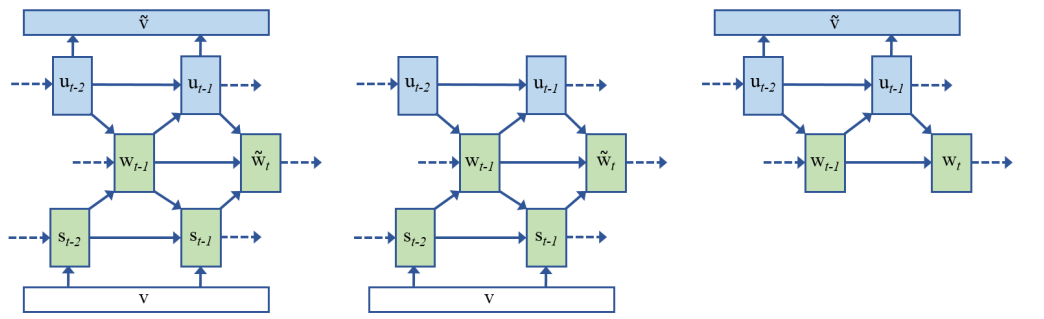
\includegraphics[scale=0.4]{Imgs/mind1.png}
	\caption{ساختار کلی شبکه ارائه شده برای نگاشت دوطرفه تصاویر و جملات در پژوهش \cite{chen2015mind}}
	\label{fig:4-mind1}
\end{figure}


مدل دوطرفه ارائه شده، روی سه مجموعه‌داده‌ \lr{MS COCO}، \lr{Flickr8k} و \lr{Flickr30K} آزمایش‌ شده است. برای بررسی کیفیت عمل‌کرد مدل، باید در دو آزمایش مجزا، کیفیت نگاشت تصاویر به جملات و همین‌طور کیفیت نگاشت جملات به تصاویر توسط مدل، مورد بررسی قرار گیرند. در این قسمت قصد داریم با گزارش نتایج آزمایشات در قالب جداول و تصاویر، به بررسی عمل‌کرد مدل بپردازیم. 
\\
در جدول \ref{tbl:4-mind1}، مدل \lr{RNN + IF\enfootnote{Image Feature}} یک شبکه عصبی بازگشتی است که ویژگی‌های استخراج شده از تصویر نیز به عنوان ورودی به آن داده شده است. مدل \lr{RNN + FT\enfootnote{Fine Tuned}} شبکه عصبی با ورودی بردار ویژگی تصویر است که در آن خطای ایجاد شده از خروجی شبکه بازگشتی، به شبکه کانولوشنی نیز منتقل می‌شود و وزن‌های دوشبکه بازگشتی و کانولوشنی با هم به‌روزرسانی می‌شوند.


\begin{table}[h]
	\centering
	\caption{امتیاز \lr{BLEU} کسب شده توسط مدل نگاشت دوطرفه ارائه شده در مقایسه با مدل‌های دیگر \cite{chen2015mind}.}
	\label{tbl:4-mind1}
	\begin{tabular}{|c|c|c|c|}
		\hline
		نام مدل&  \lr{‌Flickr8k} & \lr{‌Flickr30k} &\lr{‌MS COCO} 
		\\
		\hline
		\lr{RNN} & 4.5  & 6.3 & 4.7 \\
		\lr{RNN + IF}  & 11.9  & 11.3& 16.3 \\
		\lr{RNN + IF + FT}  & 12.0 & 11.6 & 17.0 \\
		\lr{RNN + VGG}  & 12.4 & 11.9 &18.4 \\
		\hline
		روش ارائه شده & \ 12.2  & 11.3 &  16.3 \\
		روش ارائه شده\lr{ + FT}  & 12.4 & 11.6 &  16.8 \\
		روش ارائه شده\lr{ + VGG} & 13.1 & 12.0 & 18.8 \\
		\hline
		انسان & 20.6 & 18.9 & 19.2\\
		\hline
	\end{tabular}
	
\end{table}


علاوه بر جدول فوق که نتایج عمل‌کرد مدل پیشنهادی را در قالب میزان امتیاز \lr{BLEU} نمایش داده و با مدل‌های دیگر مقایسه می‌کند، برای بررسی کیفیت عمل‌کرد مدل، شکل \ref{fig:4-mind1p} جملات تولید شده مدل را با جملات نوشته شده توسط عوامل انسانی مورد مقایسه قرار می‌دهد. جملات قرمز رنگ در این تصویر، جملاتی هستند که توسط مدل ارائه شده تولید شده‌اند و جملات مشکی‌رنگ، جملاتی هستند که توسط عوامل انسانی نوشته‌شده‌اند. سطر آخر در این تصویر، نشان‌دهنده تعدادی از نمونه‌هایی است که در آن‌ها جملات تولید شده توسط مدل، دچار خطا شده‌اند.



\begin{figure}[h]
	\centering
	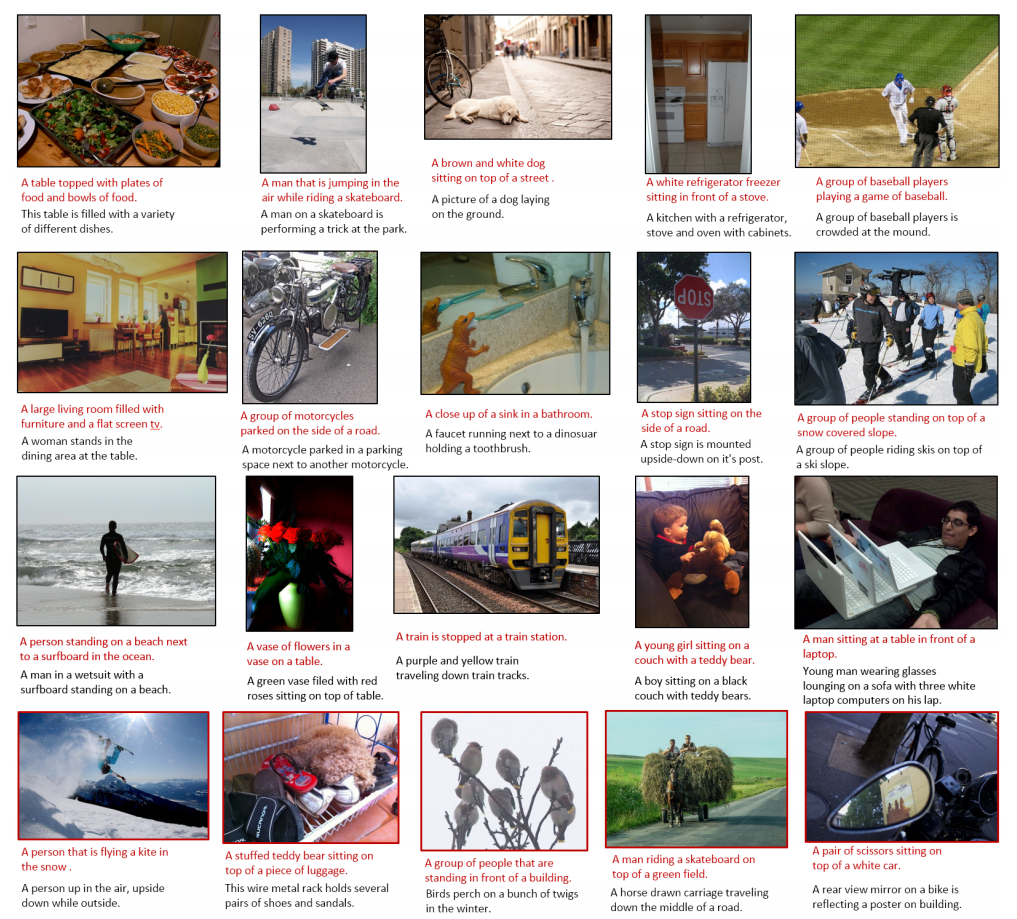
\includegraphics[scale=0.4]{Imgs/mindsEyeRes1.png}
	\caption{نمونه‌ای از جملات تولید شده برای تصاویر توسط مدل پیشنهاد شده در \cite{chen2015mind}}
	\label{fig:4-mind1p}
\end{figure}


علاوه بر موارد فوق، جدول \ref{tbl:4-mind2} نتایج بازیابی تصاویر با وارد کردن جمله را در این مدل با مدل‌های دیگر مورد مقایسه قرار می‌دهد. در مدل‌های ارائه شده در این جدول، استفاده از عبارت \lr{T} در انتهای نام مدل، بیان‌گر این نکته است که در مدل مشخص شده، جملات بر اساس درست‌نمایی آن‌ها با داشتن تصویر ورودی مرتب شده‌اند. به علاوه، استفاده از عبارت  \lr{I} در نام مدل‌ها نمایان‌گر این نکته است که در این مدل‌ها، از خطای بازسازی تصویر نیز برای مرتب‌سازی جملات خروجی استفاده شده است.


\begin{table}[h]
	\centering
	\caption{جدول نتایج بازیابی تصاویر با استفاده از جملات ورودی در مدل ارائه شده در \cite{chen2015mind}}
	\label{tbl:4-mind2}
	\begin{tabular}{|c|c|c|c|c|}
		\hline
		نام مدل& \lr{R@1} & \lr{R@5} & \lr{R@10} & \lr{Med r 500}\\
		\hline
		\lr{M-RNN} & 12.6 & 31.2& 41.5& 16 \\
		\lr{RNN + VGG} & 15.1 & 41.1 & 54.1 & 9 \\
		روش ارائه شده \lr{T} & 17.7 & 44.9 & 57.2 & 7.5 \\
		روش ارائه شده \lr{T + I} & 18.5 & 45.7 & 58.1 & 7\\
		\hline
	\end{tabular}
\end{table}



%%%%%%%%%%%%%%%%%%%%%%%%12345%%%%%%%%%%
\section{تولید شرح بر تصاویر با استفاده از روش‌های مبتنی بر توجه بصری}
ایده‌ اصلی روش‌های مبتنی بر توجه بصری از پژوهش‌های موجود در زمینه ترجمه ماشینی گرفته شده است. این دسته از پژوهش‌ها مدلی ارائه می‌دهند که با استفاده از آن بتوان هر کلمه از جملات تولیدی را با تمرکز بر یک یا بخشی از کلمات موجود در جمله مبدا‌، تولید کرد. به طور مشابه، در حوزه تولید خودکار شرح بر تصاویر، از این دسته از پژوهش‌ها به منظور حصول مدلی استفاده می‌شود که قادر باشد هر یک از کلمات موجود در جمله را با استفاده از بخشی از تصویر ورودی، تولید نماید.
\\
در این فصل، ابتدا ایده اصلی ترجمه مبتنی بر توجه بصری را در حوزه ترجمه ماشینی ارائه خواهیم کرد و سپس کاربردهای این ایده را در حوزه تولید خودکار شرح بر تصاویر مورد بررسی قرار می‌دهیم. 

\subsection{روش‌های مبتنی بر توجه بصری در حوزه ترجمه ماشینی}

همان‌طور که گفته شد، تمام روش‌های قبلی را می‌توان به دو مرحله زیر تقسیم کرد.
\begin{enumerate}
	\item نگاشت نمونه‌ها از فضای تصاویر به فضای ویژگي‌ها
	\item نگاشت نمونه‌ها از فضای ویژگی‌ها به فضای جملات
\end{enumerate}

در حوزه ترجمه ماشینی، به تابع نگاشت مرحله اول، رمزگذار\enfootnote{Encoder} و به تابع نگاشت مرحله دوم، رمزگشا\enfootnote{Decoder} گفته می‌شود. در این بخش، ما از این عبارات برای ارجاع به مراحل اول و دوم الگوریتم استفاده می‌نماییم.
\\
چارچوب کاری رمزگذار-رمزگشا، در تعداد زیادی از پژوهش‌های حوزه ترجمه ماشینی به عنوان چارچوب کاری اصلی مورد استفاده قرار گرفته است. تمام روش‌های قبلی که در فصول قبل ذکر شد نیز از همین چارچوب کاری به عنوان چارچوب اصلی بهره برده‌اند. به عنوان مثال در روش‌های مبتنی بر یادگیری عمیق برای تولید خودکار شرح بر تصاویر از شبکه‌های عصبی کانولوشنی به طور معمول به عنوان رمزگذار و از شبکه‌های عصبی بازگشتی به عنوان رمزگشا استفاده می‌شود.
\\
شکل \ref{fig:5-1} نشان‌دهنده ساختار کلی چارچوب کاری رمزگذار-رمزگشا است.

\begin{figure}[h]
	\centering
	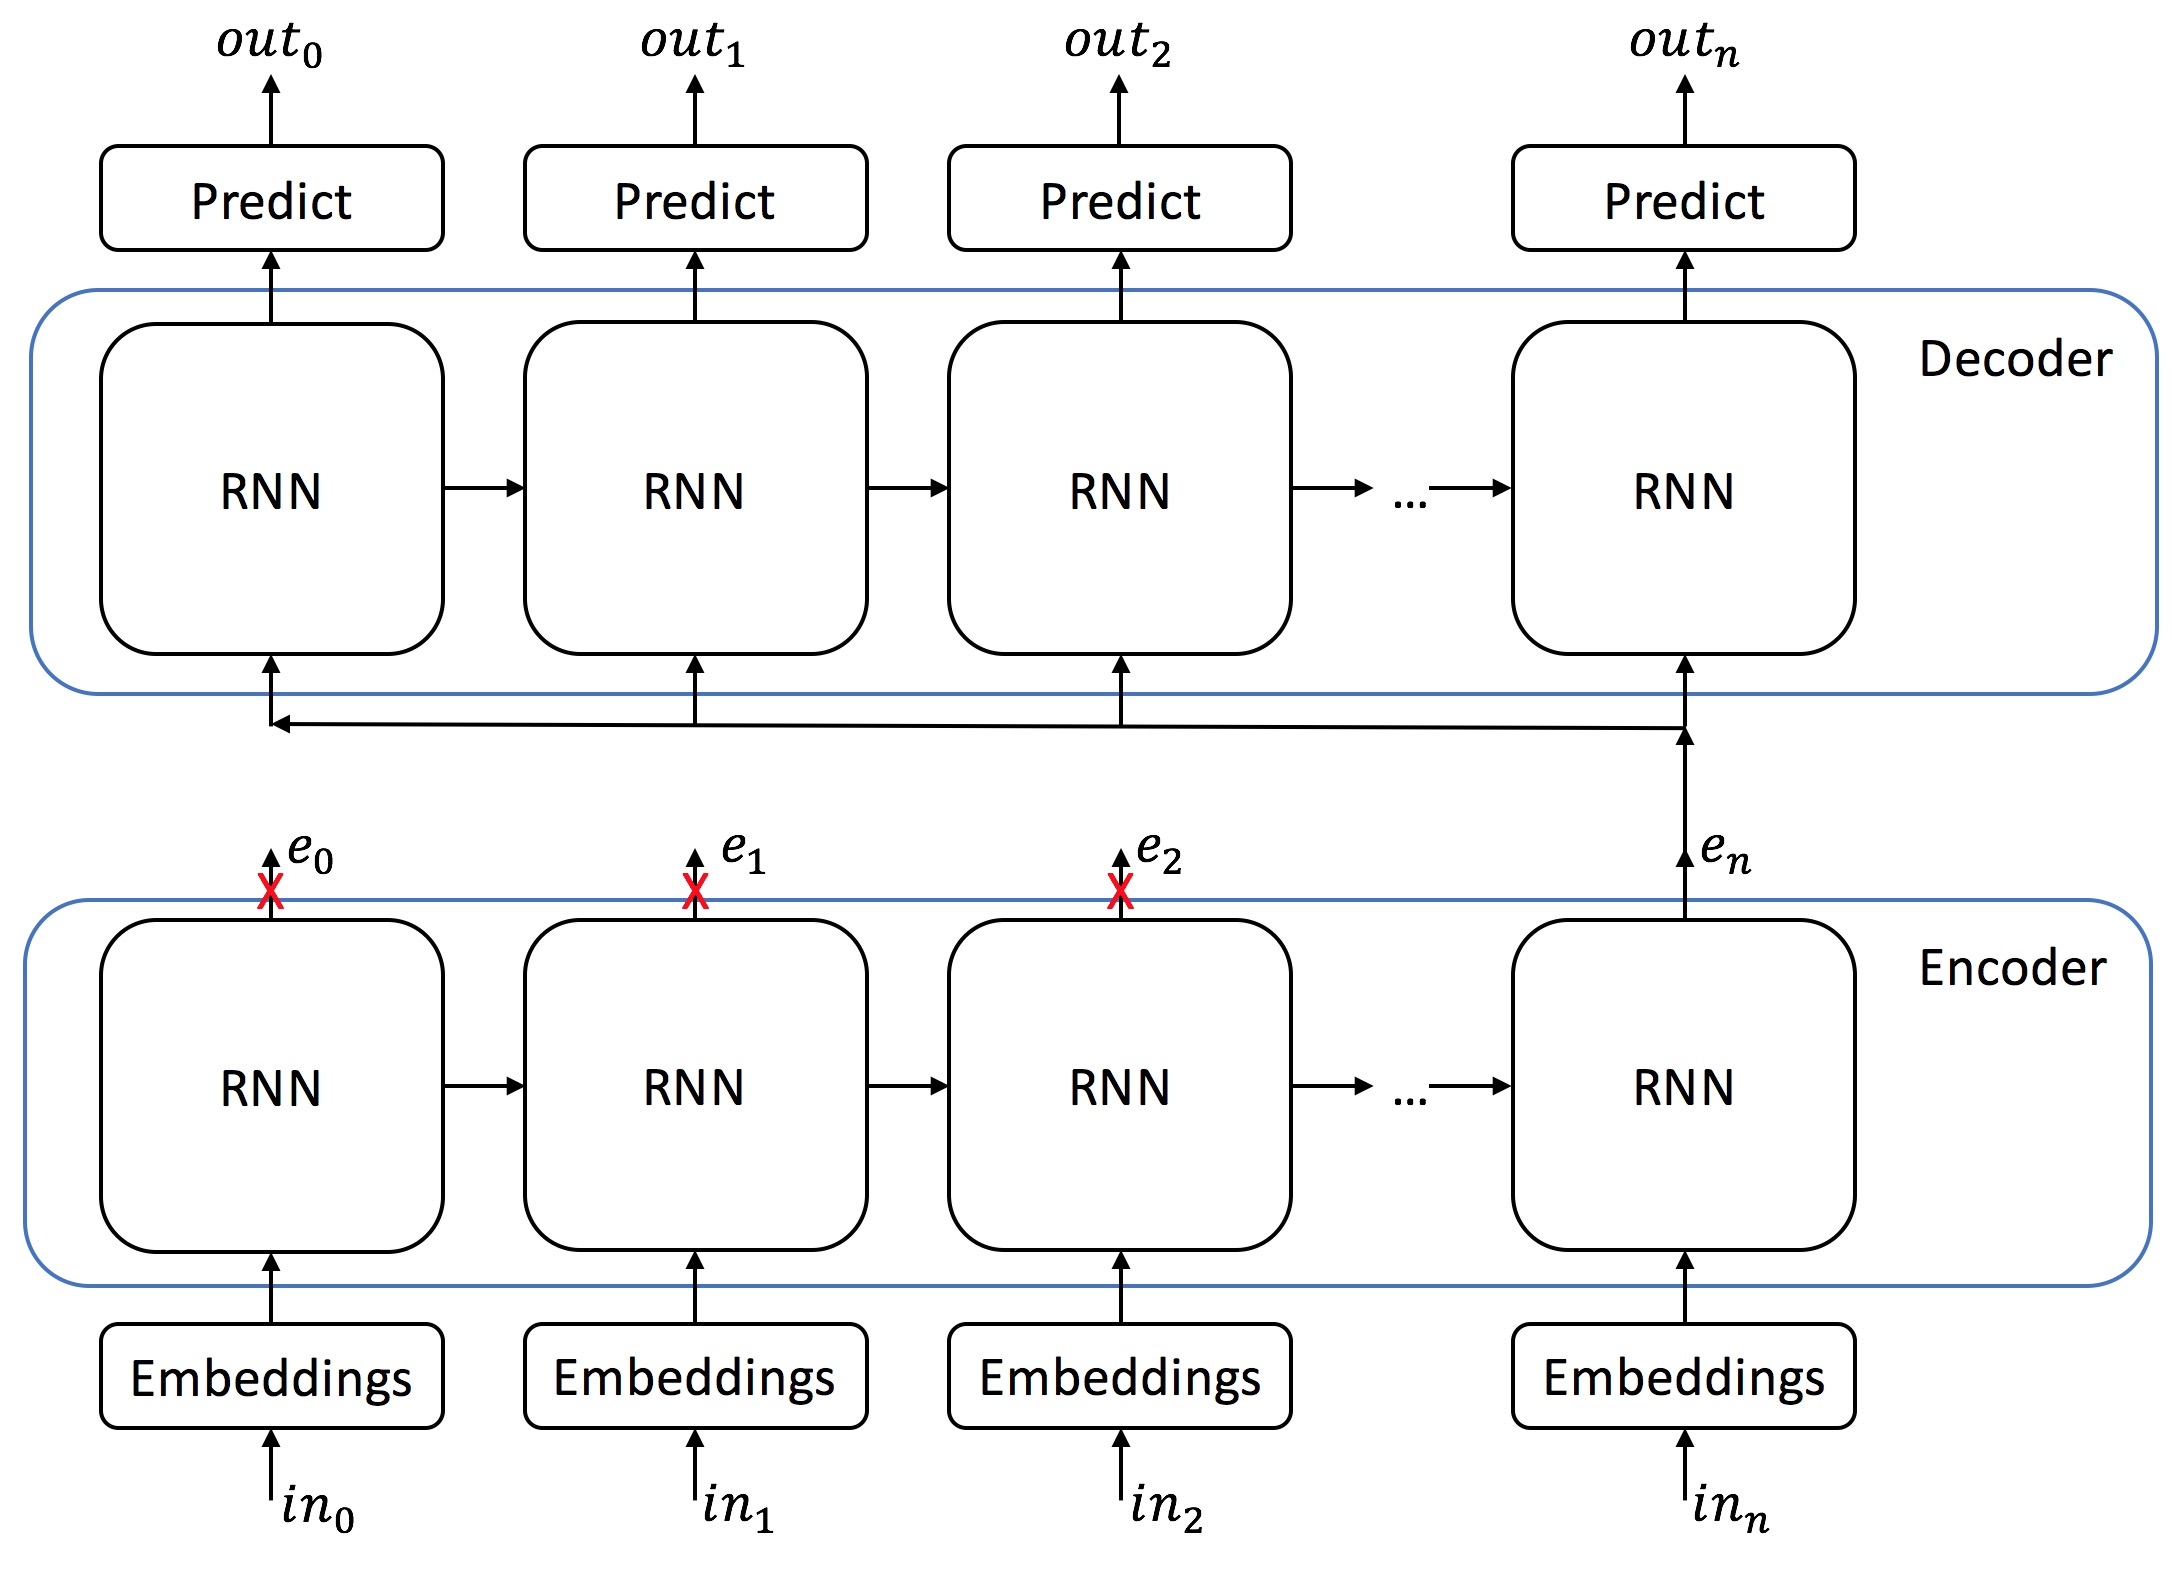
\includegraphics[scale=0.2]{Imgs/encoder-decoder.jpg}
	\caption{ساختار کلی چارچوب کاری رمزگذار-رمزگشا}
	\label{fig:5-1}
\end{figure}


در ادامه به بررسی بخش‌های مختلف این چارچوب کاری می‌پردازیم و سپس ایده اصلی روش‌های مبتنی بر توجه بصری را که توسط آقای بنجیو در پژوهش \cite{bahdanau2014neural} در سال 2014 ارائه شده است، مورد بررسی قرار خواهیم 
داد.


\subsubsection{رمزگذار}
رمزگذار در این چارچوب کاری، با گرفتن یک جمله به عنوان ورودی، بردار ویژگی متناظر جمله مبدا را تولید می‌کند. جمله ورودی با دنباله‌ای از کلمات مدل می‌شود. همین‌طور هر کلمه را با یک بردار $n$ بعدی، که $n$ تعداد کلمات موجود در دیکشنری است، مدل می‌شود. به این ترتیب، هر جمله ورودی، یک بردار با طول متغیر است که هر مولفه آن خودش برداری به ابعاد  $n$ است. از طرفی بردار خروجی، که همان بردار ویژگی‌ها است، یک بردار با طول ثابت و قراردادی خواهد بود.
\\
عموما در کاربردهای ترجمه ماشینی در هر دو بخش رمزگذار و رمزگشا از شبکه‌های عصبی بازگشتی استفاده می‌شود. در شبکه‌های عصبی بازگشتی، خروجی هر مرحله تابعی از ورودی آن مرحله و حالت شبکه در مرحله جاری است. با فرض این‌که $h_t$ حالت شبکه در زمان $t$ را نمایش دهد می‌توان رابطه تولید خروجی توسط شبکه عصبی بازگشتی را مطابق با \eqref{eq:5-1} تعریف نمود.
\begin{align*}
	h_t& = f(X_t , h_{t-1}) \\
	C& = q(h_1, \cdots, h_L)
	\numberthis 
	\label{eq:5-1}
\end{align*}
به طور معمول از شبکه 
\lr{LSTM}
به عنوان تابع $f$ استفاده می‌شود و همین‌طور به جای استفاده از تابع $q$ حالت نهایی شبکه به عنوان بردار ویژگی مورد استفاده قرار می‌گیرد
\cite{bahdanau2014neural}.

\subsubsection{رمزگشا}

رمزگشا به منظور نگاشت فضای ویژگی‌ها به فضای جملات مورد استفاده قرار می‌گیرد. خروجی رمزگذار، ورودی رمزگشا است. با این فرض، ورودی رمزگشا یک بردار ویژگی با طول ثابت است و خروجی آن که یک جمله به زبان مقصد است، همانند جمله مبدا، یک بردار با طول متغیر شامل بردارهای بازنمایی کلمات است. رمزگشا در اصل در هر مرحله، به دنبال یافتن کلمه‌ای است که با داشتن کلمات تولید شده قبلی و بردار ویژگی موجود، محتمل‌ترین کلمه نسبت به بقیه کلمات موجود در دیکشنری باشد. تابع احتمال مربوطه را می‌توان به فرم \eqref{eq:5-2} تعریف نمود.

\begin{equation}
p(y_t | C, y_1, y_2, \cdots, y_{t-1}) = g(y_t, s_t, C)
\label{eq:5-2}
\end{equation}

در رابطه \eqref{eq:5-2}، $C$ نشان‌دهنده بردار ویژگی‌، $y_i$ نشان‌دهنده لغت $i$ام تولید شده از زبان مقصد و بردار $s_t$ نشان‌دهنده حالت شبکه بازگشتی مورد استفاده به عنوان رمزگشا است.


شکل \ref{fig:decoder} ساختار کلی رمزگشا را نمایش می‌دهد.

\begin{figure}[h]
	\centering
	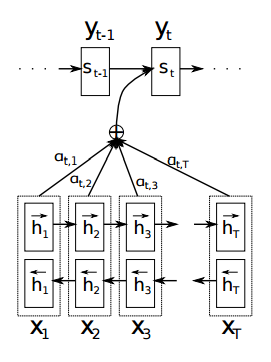
\includegraphics[scale=0.7]{Imgs/5-decoder.png}
	\caption{ساختار رمزگشا مورد استفاده در چارچوب کاری \cite{bahdanau2014neural}}
	\label{fig:decoder}
\end{figure}

\subsubsection{ایده اصلی استفاده از توجه بصری}

همان‌طور که بیان شد، در چارچوب کاری رمزگذار-رمزگشا، ابتدا جمله ورودی که شامل تعداد نامعلوم کلمه است به یک بردار با طول متغیر مدل می‌شود. بردار تولید شده توسط یک رمزگذار به یک بردار با طول ثابت، که همان بردار ویژگی‌ها است، نگاشت شده و در نهایت بردار ویژگی تولید شده توسط یک رمزگذار به یک بردار با طول متغیر که نماینده جمله زبان مقصد است، نگاشت می‌شود.
\\
فرآیند مذکور یک محدودیت جدی دارد و آن این است که رمزگذار باید بتواند تمام اطلاعات مورد نیاز برای تولید جمله را در یک بردار با طول ثابت بگنجاند و رمزگشا باید بتواند تمام اطلاعات مورد نیاز خود را از همین بردار با موجود با طول ثابت، استخراج کند. این محدودیت باعث می‌شود قدرت کد کردن اطلاعات در بردار ویژگی کاهش یابد. برای حل این مشکل از ایده نقاط توجه استفاده می‌نماییم.
\\
در این دسته از روش‌ها به جای این‌که رمزگذار فقط یک بردار ویژگی تولید کند، بردارهای ویژگی مختلفی ایجاد می‌کند که هر بردار با تمرکز بر روی یک یا بخشی از جمله مبدا تولید شده است. به این ترتیب، هر بردار تولید شده شامل اطلاعات معنایی یک یا بخشی از جمله مبدا می‌باشد. به این طریق، رمزگشا می‌تواند با انتخاب بین بردارهای معنایی تولید شده در هر مرحله، کلمه تولیدی را با تمرکز بر روی معنای یک کلمه و کلمات مجاور آن در جمله مبدا، تولید کند.
\\
در ادامه به بررسی تغییراتی که باید در رمزگذار و رمزگشا اتفاق بیفتد تا بتوان به جای یک بردار ویژگی مجموعه‌ای از بردارهای ویژگی با تمرکز محلی ایجاد نمود و از آن‌ها برای تولید جمله استفاده نمود را مورد بررسی قرار می‌دهیم. برای سهولت فهم تغییرات، ابتدا تغییرات رمزگشا را مطرح نموده و سپس به بررسی تغییرات رمزگذار خواهیم پرداخت.
\subsubsection{رمزگشا در روش مبتنی بر توجه بصری}
فرض می‌کنیم به جای تنها یک بردار ویژگی، $L$ بردار ویژگی از ورودی استخراج شده باشد. آن‌ها را در یک ماتریس به شکل $C = [c_1, \cdots, c_L]^T$ بازنمایی می‌نماییم. فرض می‌کنیم بردار ویژگی $c_i$ به دنباله حاشیه‌نویسی‌های\enfootnote{Annotation} $h = [h_1, \cdots, h_L]^T$ وابسته است. حاشیه‌نویسی $h_i$ خود یک متغیر تصادفی به شکل برداری است که دارای دو ویژگی بسیار مهم می‌باشد.
\begin{enumerate}
	\item .حاوی اطلاعات استخراج شده از تمام جمله است
	\item تمرکز استخراج اطلاعات بر روی کلمه $i$ام و کلمات اطراف آن بوده است.
\end{enumerate}
با تعریف این دو ویژگی، حاشیه‌نویسی‌ها را می‌توان همان بردار ویژگی جمله تصور کرد با این شرط که علاوه بر این که معنای کل جمله را کد کرده‌اند، تمرکز بیشتری بر معنای کلمه $i$ام و کلمات مجاور آن دارند. به عبارت بهتر هر حاشیه‌نویسی علاوه بر این‌که معنای کلی جمله را کد می‌کند، حاوی معنای محلی مربوط به کلمات هم هست.
\\
با تعریف حاشیه‌نویسی به شکل فوق و با تکیه بر فرض‌های انجام شده، می‌توانیم مدل احتمالاتی ارائه شده را به شکل  \eqref{eq:5-3} تغییر دهیم. 
\begin{equation}
p(y_i| y_1, \cdots, y_{i-1}, X) = g(y_{i-1}, S_i, c_i)
\label{eq:5-3} 
\end{equation}
که در آن:
\begin{align*}
	c_i = \Sigma_{j=1}^L \alpha_{ij}h_j
	\numberthis
	\label{eq:5-4}
	\\
	\alpha_{ij} = \frac{exp(e_{ij})}{\Sigma_{k=1}^Lexp(e_{ik})}
	\numberthis
	\label{eq:5-5}
	\\
	e_{ij} = f(s_{i-1}, h_j)
	\numberthis
	\label{eq:5-6}
\end{align*}

متغیر تصادفی $e_{ij}$ که در رابطه \eqref{eq:5-6} تعریف شده است نمایان‌گر میزان شباهت کلمه $i$ام در جمله خروجی به کلمه $j$ام در جمله ورودی است. وظیفه‌ این متغیر، هم‌ترازسازی\enfootnote{Alignment} ورودی و خروجی است. $\alpha_{ij}$ یک نرمال‌سازی روی امتیازهای محاسبه شده انجام می‌دهد. از این متغیر نرمال شده به عنوان وزن حاشیه‌نویسی‌ها استفاده می‌شود. مطابق با رابطه \eqref{eq:5-4} بردار ویژگی مورد استفاده برای تولید کلمه در جمله مقصد، از طریق یک میانگین‌گیری بر اساس وزن معنایی کلمات تولید می‌شود.
\\
در رابطه \eqref{eq:5-6} $s_{i-1}$ بردار حالت شبکه رمزگشا در زمان $i-1$ و $f$ یک تابع امتیاز است. تابع امتیاز مورد استفاده در این رابطه را می‌توان با یک شبکه عصبی پیش‌رو\enfootnote{Feed Forward Neural Network} مدل‌سازی کرد. در صورت استفاده از شبکه عصبی پیش‌رو برای مدل‌سازی تابع شباهت، در صورتی که از هم‌ترازسازی نرم\enfootnote{Soft Alignment} استفاده شود، تابع هدف مشتق‌پذیر شده و می‌توانیم از الگوریتم پس‌انتشار خطا برای آموزش استفاده نماییم.


\subsubsection{رمزگذار در روش مبتنی بر توجه بصری}
برای طراحی رمزگذار در این بخش، باید مکانیزمی ارائه شود که قادر باشد حاشیه‌نویسی‌های $h_1$ تا $h_L$ را طوری تولید کند که دو شرط مطرح شده در بخش قبلی را ارضا نمایند. به عبارت دیگر باید بردارهای ویژگی‌ای استخراج نماییم که علاوه بر این‌که حاوی معنای کل جمله باشند، هر یک از آن‌ها بر روی معنای یک کلمه و کلمات اطراف آن تمرکز بیشتری نسبت به سایر بردارها داشته باشند تا بتوانیم علاوه بر مدل‌سازی معنای کلی جمله، از معنای محلی کلمات هم استفاده نماییم.
\\
به این منظور از یک شبکه عصبی بازگشتی دوطرفه در مدل‌سازی رمزگذار استفاده می‌نماییم. شکل \ref{fig:biencoder} ساختار کلی یک شبکه عصبی بازگشتی دوطرفه را نمایش می‌دهد. 

\begin{figure}[h]
	\centering
	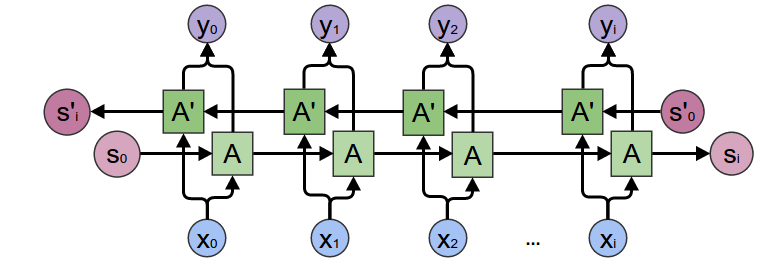
\includegraphics[scale=0.6]{Imgs/biencoder.png}
	\caption{ساختار کلی یک شبکه عصبی بازگشتی دوطرفه}
	\label{fig:biencoder}
\end{figure}

همان‌طور که در شکل \ref{fig:biencoder} مشخص است، یک شبکه عصبی بازگشتی دوطرفه شامل دو شبکه پیش‌رو در خلاف جهت یک‌دیگر است. حالت‌های مخفی شبکه پیش‌رو رو به راست را با $h_i^\rightarrow$ و حالت‌های مخفی شبکه پیش‌رو رو به چپ را با $h_i^\leftarrow$ نمایش می‌دهیم. همان‌طور که در شکل پیداست، خروجی‌های شبکه در این ساختار هم به حالت‌های سمت راست و کلمات سمت راست در جمله و هم به حالات و کلمات سمت چپ وابسته هستند. پس همین خروجی‌ها را می‌توان به عنوان حاشیه‌نویسی‌هایی که هر دو ویژگی را دارند مورد استفاده قرار داد.
یکی از راه‌های ساده برای ایجاد حاشیه‌نویسی با استفاده از حالات شبکه‌های پیش‌رو رو به راست و رو به چپ این است که مطابق با رابطه \eqref{eq:5-7} با پشت سر هم قرار دادن حالات شبکه، حاشیه‌نویسی مورد نیاز را تولید نماییم.
\begin{equation}
h_j = [{h_j^\rightarrow}^T, {h_j^\leftarrow}^T]^T
\label{eq:5-7}
\end{equation}



\subsection{روش‌های مبتنی بر توجه بصری در حوزه تولید شرح متناظر تصویر}
در بخش قبل به بیان ایده اصلی روش‌های مبتنی بر توجه بصری در حوزه ترجمه ماشینی پرداختیم. ساختار کلی رمزگذارها و رمزگشاها در این قالب و همین‌طور نحوه تولید بردارهای ویژگی مختلف از جمله مبدا و استفاده از این بردارها در تولید جمله مقصد را مورد بررسی قرار دادیم. در این بخش  به بررسی پژوهش‌هایی خواهیم پرداخت که از این ایده در حوزه تولید شرح متناظر تصویر بهره‌ جسته‌اند.
\\
یکی از برجسته‌ترین و مورد توجه‌ترین پژوهش‌ها از این دست، پژوهشی است که آقای بنجیو و همکارانش در سال 2015 ارائه داده‌اند
\cite{xu2015show}.
در این بخش به بررسی این پژوهش خواهیم پرداخت.

\subsubsection[تولید شرح متناظر تصویر با استفاده از توجه بصری و شبکه‌های عصبی]{تولید شرح متناظر تصویر با استفاده از توجه بصری و شبکه‌های عصبی \cite{xu2015show}}

در این پژوهش که در سال 2015 توسط آقای بنجیو و همکارانش ارائه شده است از ایده استفاده از توجه در حوزه ترجمه ماشینی استفاده شده است تا شرح متناظر تصاویر با دقت بیشتری تولید شود. چارچوب کاری رمزگذار-رمزگشا مانند آن‌چه در بخش قبلی مطرح شد در این پژوهش مورد استفاده قرار گرفته است.
\\
رمزگذار ارائه شده در این پژوهش، یک شبکه عصبی کانولوشنی است که قادر به تولید $L$ بردار ویژگی مختلف است. به هر یک از این بردارهای ویژگی یک حاشیه‌نویسی\enfootnote{Annotation} تصویر گفته می‌شود. بردارهای حاشیه‌نویسی، همان‌طور که در بخش قبل ذکر شد، باید دارای دو شرط زیر باشند:
\begin{enumerate}
	\item حاوی معنای تصویر به طور کلی باشند.
	\item تمرکز بیشتری روی یکی از بخش‌های تصویر داشته باشند.
\end{enumerate}
برای این‌که بتوانیم دو شرط فوق را در بردارهای حاشیه‌نویسی تولید شده از رمزگذار بگنجانیم از خروجی لایه ما قبل آخر شبکه عصبی کانولوشنی به عنوان بردارهای حاشیه‌نویسی استفاده می‌کنیم. هر بردار حاشیه‌نویسی یک بردار $D$ بعدی است که مربوط به یک بخش از تصویر می‌شود و آن را با $a_i$ نمایش می‌دهیم. بنابر این داریم:
\begin{equation}
a = \{a_1, a_2, \cdots, a_L\}, a_i \in R^D
\end{equation}

در این پژوهش از یک شبکه حافظه کوتاه‌مدت بلند به عنوان رمزگشا استفاده شده است. این شبکه با دریافت مجموعه بردارهای حاشیه‌نویسی $a$، جمله‌ای به زبان انگلیسی تولید می‌کند که شامل دنباله‌ای از $C$ کلمه است. هر کلمه با یک بردار $K$ بعدی نمایش داده می‌شود که $K$ تعداد کلمات موجود در دیکشنری است. در هر یک از بردارهای بازنمایی کلمات فقط یک مولفه یک است و مابقی مولفه‌ها صفر هستند. مولفه‌ای که برابر با یک است نمایش‌دهنده اندیس کلمه در دیکشنری است.
\\
شکل \ref{fig:satenc} یک سلول از شبکه حافظه کوتاه‌مدت بلند مورد استفاده در این پژوهش به عنوان رمزگشا را نمایش می‌دهد. 
\begin{figure}[h]
	\centering
	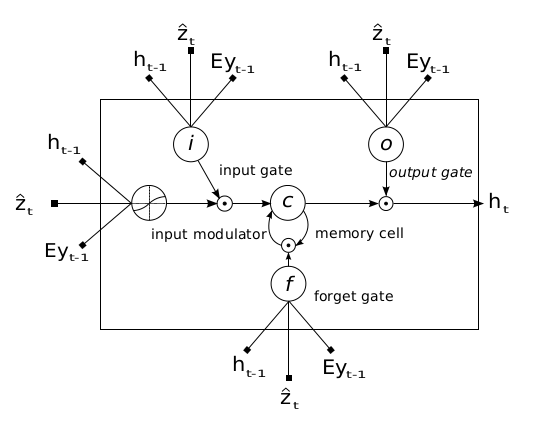
\includegraphics[scale=0.6]{Imgs/satenc.png}
	\caption{یک واحد از شبکه حافظه کوتاه‌مدت بلند مورد استفاده در رمزگشا پژوهش \cite{xu2015show}}
	\label{fig:satenc}
\end{figure}
روابط مربوط به یادگیری این شبکه را می‌توان مطابق با روابط \eqref{eq:5-8} تا \ref{eq:5-13}  نمایش داد. در همه روابط، تابع $T$ یک تابع نگاشت خطی به شکل $T: R^{D+m+n}*R^n$ است که پارامترهای آن آموزش داده‌ شده‌اند. متغیر $i_t$ ورودی، $f_t$ خروجی سلول فراموشی، $c_t$ حافظه، $o_t$ خروجی و $h_t$ حالت مخفی شبکه را نمایش می‌دهند. 
\begin{align*}
	i_t &= \sigma(T(Ey_{t-1}, h_{t-1}, \hat{z}_{t-1})) \numberthis \label{eq:5-8} \\
	f_t &= \sigma(T(Ey_{t-1}, h_{t-1}, \hat{z}_{t-1})) \numberthis \label{eq:5-9} \\
	o_t &= \sigma(T(Ey_{t-1}, h_{t-1}, \hat{z}_{t-1})) \numberthis \label{eq:5-10} \\
	g_t &= \sigma(T(Ey_{t-1}, h_{t-1}, \hat{z}_{t-1})) \numberthis \label{eq:5-11} \\
	c_t &= f_t \odot c_{t-1} + i_t \odot g_t \numberthis \label{eq:5-12} \\
	h_t &= o_t \odot tanh(c_t) \numberthis \label{eq:5-13} \\
\end{align*}

بردار $\hat{z}_{t-1}$ بردار معنای تصویر را نمایش می‌دهد که با استفاده از بردارهای حاشیه‌نویسی تولید شده در رمزگذار تولید می‌شود. ماتریس $E$، ماتریس جانمایی\enfootnote{Embedding Matrix} به ابعاد $m * K$ است. تابع $\sigma$ تابع فعالیت سیگموئیدی و $\odot$ حاصل‌ضرب مولفه‌های نظیر به نظیر بردارها را نمایش می‌دهند.
\\
فرایند آموزش رمزگشا کاملا مطابق با فرایند آموزش معمول شبکه حافظه کوتاه‌مدت بلند است. تنها تفاوت در این پژوهش وجود و نحوه محاسبه بردار معنای $\hat{z}_{t-1}$  است که توجه بصری را تعریف می‌کند. برای محاسبه این متغیر تابع $\phi$ را تعریف می‌نماییم. این تابع در هر لحظه از زمان با استفاده از مجموعه بردارهای حاشیه‌نویسی $a$ برداری تولید می‌کند که به عنوان بردار ویژگی‌ استخراج شده از تصویر در هر لحظه مورد استفاده قرار می‌گیرد.
\\
تابع $phi$ می‌تواند به دو شکل بردار ویژگی را تولید نماید. روش اول این است که ابتدا با تولید وزن‌های مثبت $\alpha_i$ برای هر ناحیه از تصویر با بردار حاشیه‌نویسی $a_i$ یک احتمال برای میزان مناسب بودن ناحیه $i$ از تصویر برای استفاده در تولید کلمه در زمان $t$ تعریف شود. سپس بردار حاشیه‌نویسی با بیشترین احتمال برای تولید کلمه انتخاب شده و به مراحل بعدی ارسال شود. این روش را تحت عنوان روش توجه سخت\enfootnote{Hard Attention} نام‌گذاری می‌نماییم.
\\
روش دوم برای تولید بردار ویژگی تصویر در هر لحظه توسط تابع $\phi$ این است که اعداد مثبت تولید شده $\alpha_i$ را به طور مستقیم به عنوان معیاری جهت سنجش میزان مناسب‌بودن نسبی نواحی نسبت به یک‌دیگر مورد استفاده قرار دهیم و با استفاده از یک میانگین‌گیری وزن‌دار بر حسب همین وزن‌های مثبت از بردارهای حاشیه‌نویسی اقدام به تولید بردار ویژگی تصویر نماییم. به این روش، روش توجه نرم \enfootnote{Soft Attention} می‌گوییم.
\\
به جهت سهولت در امر رابطه‌بندی توجه بصری در فرایند آموزش رمزگذار و رمزگشا، متغیر تصادفی $s_{t.i}$ را معرفی می‌نماییم که نشان‌دهنده این است که آیا در زمان $t$، از بردار ویژگی مربوط به ناحیه $i$ام تصویر، برای تولید کلمه استفاده می‌شود یا خیر. اگر در زمان $t$ از بردار ویژگی ناحیه $i$ام، که همان بردار حاشیه‌نویسی با اندیس $i$ است، به منظور تولید کلمه استفاده شود، مقدار متغیر $s_{t,i}$ برابر با یک و در غیر این‌ صورت برابر با صفر قرار می‌‌گیرد.
\\
با استفاده از متغیر تصادفی تعریف شده می‌توان به راحتی روابط مربوط به مدل‌سازی توجه بصری نرم و سخت را به شرح زیر تشکیل داد. نکته آخر این‌که در پژوهش مورد بررسی، به منظور تولید احتمال کلمه بعدی با توجه به کلمات تولید شده قبلی و بردار ویژگی استخراج شده از تصویر از رابطه \eqref{eq:5-131} استفاده شده است.
\begin{equation}
p(Y_t | a, Y_1^{t-1}) \propto exp(L_o(EY_{t-1} + L_h h_{t} + L_z \hat{z}_t)) 
\label{eq:5-131}
\end{equation}
در رابطه \eqref{eq:5-13} ماتریس‌های $L_o \in R^{K*m}$، $L_h \in R^{m*n}$، $L_z \in R^{m*d}$ و $E$ پارامترهای شبکه هستند که باید آموزش داده شوند.

\begin{enumerate}
	\item \textbf{توجه بصری سخت} \\
	با فرض یک توزیع \lr{Multinoulli} مطابق رابطه \eqref{eq:5-hatmult} می‌توان متغیر $\hat{z}_t$ را به عنوان بردار ویژگی استخراج‌شده نهایی با توجه به بردارهای حاشیه‌نویسی $a$ و توجه بصری بصری، به شکل رابطه \eqref{eq:5-hat} محاسبه نمود.
	
	\begin{align*}
		&p(s_{t,i} = 1 | s_{j<t}, a) = \alpha_{t,i}
		\numberthis \label{eq:5-hatmult} \\
		&\hat{z}_t = \Sigma_t s_{t,i} a_i
		\numberthis \label{eq:5-hat} 
	\end{align*}
	
	برای آموزش وزن‌های شبکه یک تابع هدف به نام $L_s$ مطابق با رابطه \eqref{eq:5-hl} مطرح می‌شود که یک کران پایین از بیشینه درستنمایی $p(Y | a)$ است که در آن $Y$ دنباله کلمات تولید شده نهایی و 
	$a$ بردارهای حاشیه‌نویسی تولید شده از روی تصویر را نمایش می‌دهند.
	
	\begin{align*}
		log\>p(Y | a) = log\> \Sigma_s\> p(s | a) p(Y | s, a) \>\geq\> \Sigma_s\> p(s | a) \>log\> p(Y | s, a) = L_s \numberthis \label{eq:5-hl} \\ 
	\end{align*}
	
	با ارائه تابع هدف $L_s$ مطابق با رابطه \eqref{eq:5-hl} و بهینه‌سازی آن می‌توان رابطه به‌روزرسانی وزن‌ها در فرایند آموزش را محاسبه نمود. رابطه \eqref{eq:5-hardatten1} محاسبات مربوطه را نمایش می‌دهد.
	
	\begin{align*}
		\frac{\partial L_s}{\partial W} = \Sigma_s p(s|a) [\frac{\partial \> log \> p(Y| s, a)}{\partial W} + log \> p(Y|s,a)\frac{\partial \> log \> p(s|a)}{\partial W}] \numberthis \label{eq:5-hardatten1}
	\end{align*}
	
	به جای متغیر $s_t$ در رابطه \eqref{eq:5-hardatten1} می‌توان با استفاده از روش نمونه‌برداری مونت‌کارلو\enfootnote{Monte Carlo Sampling} نمونه‌های تصادفی $\tilde{s_t}$ تولید کرد و سپس با استفاده از رابطه \eqref{eq:5-hardatten2} تابع هدف را بهینه نمود. 
	\begin{equation}
	\frac{\partial \> L_s}{\partial W} \approx \frac{1}{N} \Sigma_{n=1}^N [\frac{\partial \> log \> p(Y|\tilde{s}^n , a)}{\partial W} + log \> p (Y| \tilde{s}^n , a) \frac{\partial \> log \> p(\tilde{s}^n | a)}{\partial W}]
	\label{eq:5-hardatten2}
	\end{equation}
	
	\item \textbf{توجه بصری نرم} \\
	
	همان‌طور که گفته شد، تولید بردار ويژگی را می‌توان با میانگین‌گیری وزن‌دار روی بردارهای حاشیه‌نویسی انجام داد. در شرایطی که وزن‌های تخصیص داده شده به بردارهای حاشیه‌نویسی برابر صفر نباشند، توجه بصری نرم، فرایندی خواهد بود شامل تولید بردار ویژگی با استفاده از تمام حاشیه‌نویسی‌های موجود و با تمرکز روی تعدادی از حاشیه‌نویسی‌ها که ضریب بیشتری دارند. از آنجا که این شیوه محاسبه بردار ویژگی شامل یک بردار میانگین‌گیری وزن‌دار است، تمام تابع هدف مشتق‌پذیر شده و امکان استفاده از روش پس‌انتشار خطا برای یادگیری وزن‌ها فراهم می‌شود.
	\\
	در این روش به طور کلی می‌توان بردار ویژگی $\hat{z}_t$ را مطابق با رابطه \eqref{eq:5-soft1} محاسبه نمود.
	
	\begin{equation}
	E_{p(s_t | a)} [\hat{z}_t] = \Sigma_{i=1}^L \alpha_{t,i} a_i
	\label{eq:5-soft1}
	\end{equation}
	
	مطابق با رابطه \eqref{eq:5-11} حالت مخفی شبکه یک ترکیب خطی از بردار ویژگی استخراج شده از تصویر به همراه یک غیرخطی‌سازی با استفاده از تابع $tanh$ است. برای تقریب مرتبه اول حالت مخفی شبکه می‌توان از امید ریاضی بردار ویژگی $\hat{z}_t$ در رابطه \eqref{eq:5-11} استفاده کرد. با در نظر گرفتن رابطه \eqref{eq:5-13} می‌توان متغیر $n_t$ را به شکل 
	$n_t = L_o (EY_{t-1} + L_h h_t + L_z \hat{z}_t) $
	تعریف نمود. با این تعریف،‌ متغیر $n_{t,i}$ مشخص‌کننده متغیر $n_t$ است در شرایطی که $\hat{z}_t = a_i$ باشد. با استفاده از متغیر تعریف شده، میانگین هندسی وزن‌دار نرمال‌شده \enfootnote{Normalized Weighted Geometric Mean (NWGM)} را برای تولید کلمه $k$ام مطابق با رابطه \eqref{eq:5-nwgm} تعریف می‌نماییم.
	
	\begin{equation}
	NWGM[P(y_t = k | a)] = \frac{\Pi_i exp(n_{t,k,i})^{p(s_{t,i} = 1 | a)}}{\Sigma_j \Pi_i exp(n_{t,j,i})^{p(s_{t,i} = 1 | a)}} = \frac{exp(E_{p(s_{t,i}|a)}[n_{t,k}])}{\Sigma_j exp(E_{p(s_{t,i}|a)}[n_{t,j}])}
	\label{eq:5-nwgm}
	\end{equation}
	
	از آنجا که 
	$E[n_t] = L_o(EY_{t-1} + L_h E[h_t] + L_z E[\hat{z}_t])$
	، متغیر $NWGM$ می‌تواند به خوبی توسط بردار ویژگی $\hat{z}_t$ تخمین زده شود. این بدین معناست که میانگین هندسی وزن‌دار نرمال‌شده لایه نهایی شبکه می‌تواند با اعمال تابع $soft\>max$ به امید ریاضی ترکیبات خطی لایه‌های پایین‌تر محاسبه شود. 
	
	
\end{enumerate}


آزمایشات انجام شده در این پژوهش روی سه مجموعه‌داده
\lr{Flickr8k}،
\lr{Flickr30k} و
\lr{Microsoft COCO}
اجرا شده است که به ترتیب شامل 8000، 30000 و 82783 تصویر با شرح تولید‌شده توسط عوامل انسانی هستند. دو مجموعه‌داده اول برای هر تصویر، 5 شرح مختلف و مجموعه‌داده سوم در برخی تصاویر بیش از ۵ شرح را شامل می‌شوند. در تمام پژوهش‌ها به منظور یکسان‌سازی آزمایشات و نتایج، از ۵ شرح برای هر تصویر استفاده شده است. 
\\
هر دو نوع محاسبه توجه بصری در این پژوهش مورد آزمایش قرار گرفته‌اند و نتایج هریک به طور جداگانه بیان شده است. در این پژوهش از معیارهای \lr{BLEU} و \lr{METEOR} به منظور ارزیابی مدل استفاده شده است.
\\
همان‌طور که در جدول \ref{tbl:5-xures} مشخص است، در هر سه مجموعه‌داده،‌ پژوهش \cite{xu2015show} بهترین عملکرد را نسبت به روش‌های دیگر از خود نشان داده است. استفاده از توجه بصری نرم در مجموعه‌داده‌های \lr{Flickr30k} و \lr{MS COCO} عمل‌کرد بهتری نسبت به روش‌های دیگر از لحاظ معیار \lr{METEOR} از خود نشان داده‌ است. همین‌طور استفاده از توجه بصری سخت، بهترین عملکرد را در معیار \lr{BLEU} از خود نشان داده است.
\\
یکی از فعالیت‌های مفید برای بررسی نحوه عملکرد مدل که در این پژوهش مورد استفاده قرار گرفته است، بصری کردن فرایند تولید کلمه توسط مدل است. در این پژوهش، توجه بصری روی تصویر در هر مرحله به همراه کلمه تولید شده در هر مرحله مشخص شده‌اند که در درک نحوه عمل‌کرد مدل و همین‌طور پیدا کردن دلایل ایجاد کلمات غیر مرتبط بسیار کمک‌کننده هستند.  


\begin{table}[h]
	\centering
	\caption{نتایج اعمال روش \cite{xu2015show} بر روی مجموعه‌داده‌های مختلف در مقایسه با روش‌های مختلف. \cite{xu2015show}}
	\label{tbl:5-xures}
	\begin{tabular}{| c | c | c | c | c | c | c |}
		\hline
		مجموعه‌داده & نام مدل & \lr{BLEU-1} & \lr{BLEU-2} & \lr{BLEU-3} & \lr{BLEU-4} & \lr{METEOR} 
		\\
		\hline
		\hline
		\lr{Flickr8k} & \lr{Google NIC} & 63.0 & 41.0 & 27.0 & \lr{--} & \lr{--} 
		\\
		\lr{Flickr8k} & \lr{Log Bilinear} & 65.6 & 42.4 & 27.7 & 17.7 & 17.31 
		\\
		\lr{Flickr8k} & \lr{Soft Attention} & \textbf{67.0} & 44.8 & 29.9 & 19.5 & 18.93 
		\\
		\lr{Flickr8k} & \lr{Hard Attention} & \textbf{67.0} & \textbf{45.7} & \textbf{31.4} & \textbf{21.3} & \textbf{20.30} 
		\\
		\hline
		\lr{Flickr30k} & \lr{Google NIC} & 66.3 & 42.3 & 27.7 & 18.3 & \lr{--} 
		\\
		\lr{Flickr30k} & \lr{Log Bilinear} & 60.0 & 38.0 & 25.4 & 17.1 & 16.88 
		\\
		\lr{Flickr30k} & \lr{Soft Attention} & 66.7 & 43.4 & 28.8 & 19.1 & \textbf{18.49} 
		\\
		\lr{Flickr30k} & \lr{Hard Attention} & \textbf{66.9} & \textbf{43.9} & \textbf{29.6} & \textbf{19.9} & 18.46 
		\\
		\hline
		\lr{MS COCO} & \lr{CMU/MS Research} & \lr{--} & \lr{--} & \lr{--} & \lr{--} & 20.41 
		\\
		\lr{MS COCO} & \lr{MS Research} & \lr{--} & \lr{--} & \lr{--} & \lr{--} & 20.71
		\\
		\lr{MS COCO} & \lr{BRNN} & 64.2 & 45.1 & 30.4 & 20.3 & \lr{--} 
		\\
		\lr{MS COCO} & \lr{Google NIC} & 66.6 & 46.1 & 32.9 & 24.6 & \lr{--} 
		\\
		\lr{MS COCO} & \lr{Log Bilinear} & 70.8 & 48.9 & 34.4 & 24.3 & 20.03 
		\\
		\lr{MS COCO} & \lr{Soft Attention} & 70.7 & 49.2 & 34.4 & 24.3 & \textbf{23.90} 
		\\
		\lr{MS COCO} & \lr{Hard Attention} & \textbf{71.8} & \textbf{50.4} & \textbf{35.7} & \textbf{25.0} & 23.04 
		\\
		\hline
	\end{tabular}
\end{table}


شکل \ref{fig:show1} توجه بصری در هر زمان را برای تولید هر کلمه برای یک تصویر نمونه نمایش می‌دهد. ردیف بالا نمایش‌دهنده عمل‌کرد روش با استفاده از توجه بصری نرم و ردیف پایین نمایش‌دهنده عمل‌کرد روش با استفاده از توجه بصری سخت است. در این نمونه خاص، نتیجه تولید جمله برای هر دو روش یکسان بوده است.

\begin{figure}[h]
	\centering
	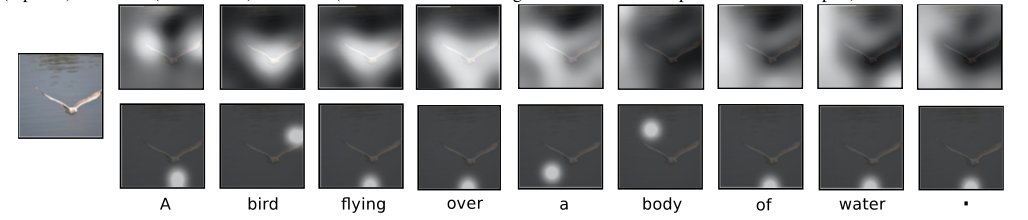
\includegraphics[scale=0.4]{Imgs/show1.png}
	\caption{نحوه عمل‌کرد الگوریتم در تغییر توجه بصری بصری و کلمه تولید شده در هر نقطه. \cite{xu2015show}}
	\label{fig:show1}
\end{figure}  

در تمام تصاویر، محدوده‌های روشن‌تر، محدوده‌هایی هستند که در آن‌ها ضریب میانگین‌گیری بیشتر بوده و توجه بیشتری در محاسبات روی آن‌ها متمرکز شده است. شکل \ref{fig:show2} چند نمونه از تصاویر را نمایش می‌دهد که در آن‌ها توجه بصری روی یک جسم منجر به تولید کلمه دقیق متناظر آن جسم شده است. کلمه تولید شده در شرح نهایی تولید شده برای تصویر در زیر هر تصویر نمایش داده شده است.

\begin{figure}[h]
	\centering
	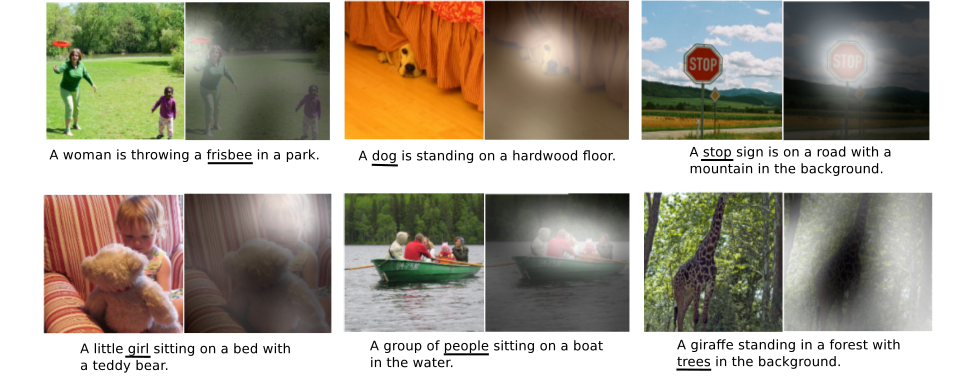
\includegraphics[scale=0.45]{Imgs/show2.png}
	\caption{چند نمونه از تصاویر که در آن‌ها توجه بصری روی یک جسم منجر به تولید کلمه دقیق متناظر شده است\cite{xu2015show}. }
	\label{fig:show2}
\end{figure}

به علاوه، شکل \ref{fig:show3} نمایش‌دهنده شرایطی است که در آن کلمه تولید شده متناظر توجه بصری بصری نیست. با استفاده از بصری‌سازی محل توجه بصری و کلمه تولید شده در هر مرحله، می‌توان به راحتی مشاهده کرد که کلمه تولید شده متناظر کدام نقطه از تصویر،‌ نامناسب است.

\begin{figure}[h]
	\centering
	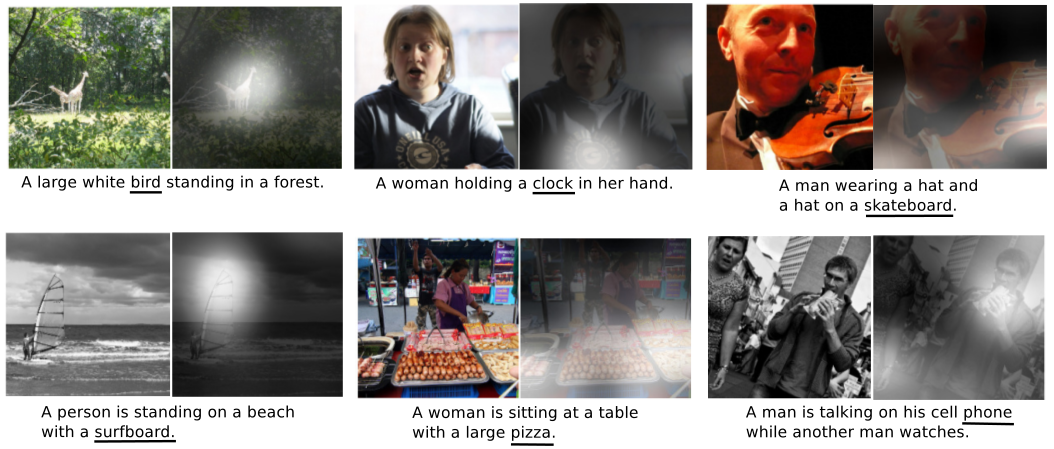
\includegraphics[scale=0.4]{Imgs/show3.png}
	\caption{نمونه‌هایی از تولید کلمات نامناسب مطابق با نقاط توجه استفاده شده در مدل‌\cite{xu2015show}}
	\label{fig:show3}
\end{figure}

علاوه بر موارد فوق، نمونه‌ای از بررسی تمام مراحل تولید شرح متناظر صحنه برای یک تصویر را در حالت‌های استفاده از توجه بصری سخت در شکل \ref{fig:show4} و توجه بصری نرم در شکل \ref{fig:show5} قابل مشاهده است. هر کلمه تولید شده در هر مرحله در کنار میزان فعال‌سازی شبکه مربوط به آن کلمه نمایش داده شده است.

\begin{figure}[h]
	\centering 
	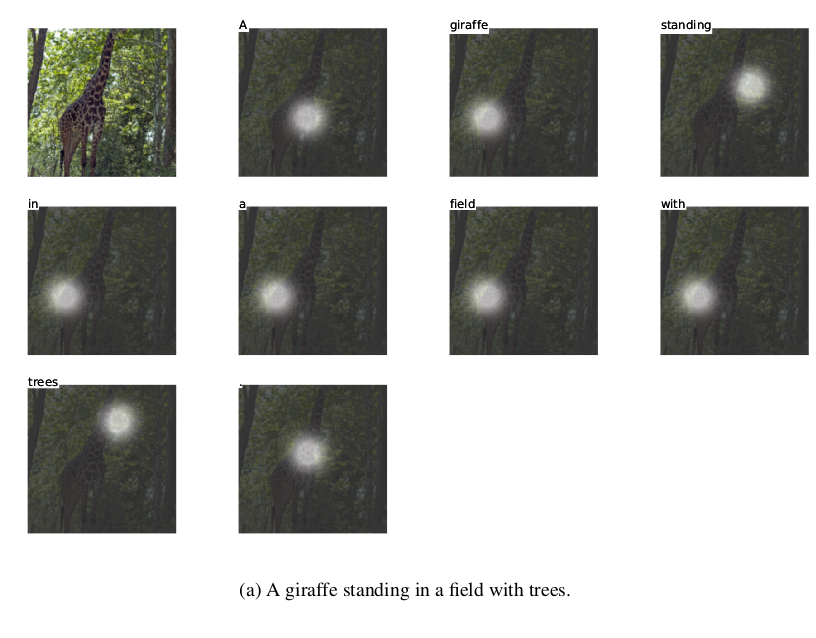
\includegraphics[scale=0.5]{Imgs/show4.png}
	\caption{فرایند تولید شرح متناظر تصویر با استفاده از توجه بصری سخت \cite{xu2015show}}
	\label{fig:show4}
\end{figure}


\begin{figure}[h]
	\centering 
	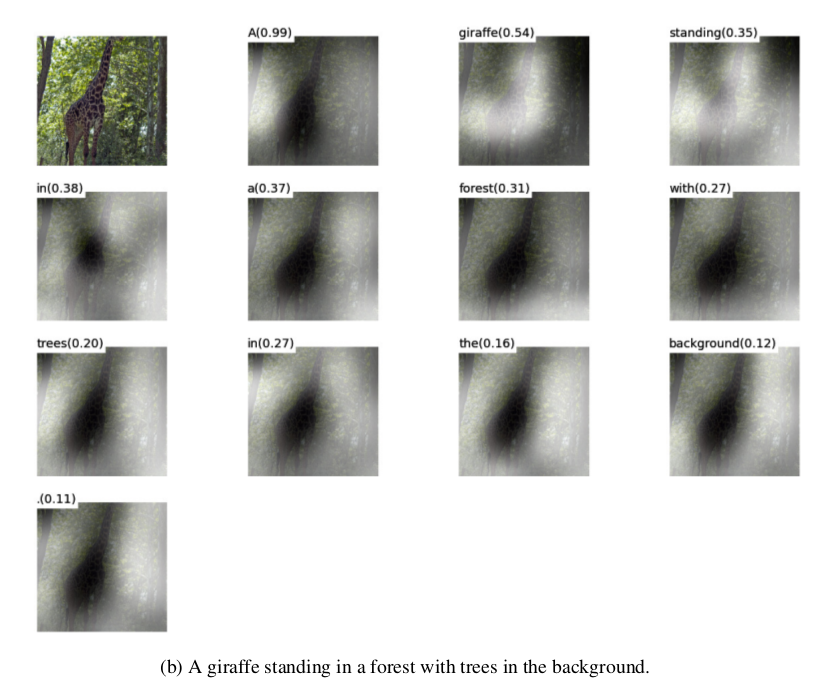
\includegraphics[scale=0.5]{Imgs/show5.png}
	\caption{فرایند تولید شرح متناظر تصویر با استفاده از توجه بصری نرم \cite{xu2015show}}
	\label{fig:show5}
\end{figure}


\subsection{فعالیت‌های مشابه دیگر}
استفاده از توجه بصری در حوزه تولید شرح متناظر تصویر، از سال 2015، توجه بسیاری از پژوهش‌گران را به خود جلب نموده است و پژوهش‌های زیادی با استفاده از این ایده سعی در تولید جمله برای تصاویر، ویدئو‌ها، صوت و انواع ورودی‌های مشابه نموده‌اند. همین‌طور در حوزه ترجمه ماشینی، نسخه‌های متفاوت و متنوعی از این ایده برای دست‌یابی به ترجمه‌های بهتر ارائه شده‌اند.
\\
یکی از پژوهش‌هایی که در این زمینه برای بهبود عمل‌کرد ترجمه ماشینی با استفاده از نقطه توجه ارائه شده است، پژوهشی است که آقای منینگ و همکارانش در سال 2015 ارائه دادند\cite{luong2015effective}.  در این پژوهش، که بر روی مجموعه‌داده \lr{WMT} که شامل جملات انگلیسی و معادل آلمانی آن‌ها است اجرا شده، از یک ساختار پشته‌ای مطابق شکل \ref{fig:5-abnmt} استفاده شده است. در این ساختار، برای آموزش، جمله انگلیسی و معادل آلمانی آن به یک‌دیگر الصاق شده و ساختار رمزگذار-رمزگشای با هم آموزش می‌بینند. سپس با دریافت ورودی جمله انگلیسی یا آلمانی، معادل آن‌ها تولید می‌شود.



\begin{figure}[h]
	\centering
	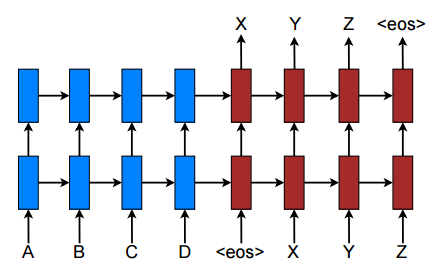
\includegraphics[scale=0.6]{Imgs/abnmt.png}
	\caption{ساختار پشته‌ای ارائه شده در \cite{luong2015effective}}
	\label{fig:5-abnmt}
\end{figure}

در پژوهش ارائه شده نیز مانند پژوهشی که آقای بنجیو در سال 2015 در حوزه ترجمه ماشینی انجام دادند، دو نوع توجه محاسبه و مورد آزمایش قرار گرفته است. توجه اول که معادل توجه نرم است، تحت عنوان توجه سراسری\enfootnote{Global Attention} و توجه دوم که معادل توجه سخت است، تحت عنوان توجه ناحیه‌ای\enfootnote{Local Attention} مطرح شده‌اند. در این آزمایش هم مشابه نتایج پژوهش \cite{xu2015show} توجه ناحیه‌ای، در بسیاری موارد عمل‌کرد بهتری نسبت به توجه سراسری از خود نشان داده‌است.
\\
پژوهش مشابهی در حوزه پرسش و پاسخ بصری توسط ایده مشابه پژوهش \cite{luong2015effective} در سال 2016 توسط آقای ینگ و همکارانش در \cite{yang2016stacked} ارائه شده است. در این پژوهش، بردار ویژگی تصویر به شرح متناظر آن که در مجموعه‌داده موجود است، الصاق شده و ساختار رمزگذار-رمزگشای به شکل مشابهی آموزش می‌بیند. سپس با ورود یک تصویر جدید، بردار ویژگی آن به ساختار داده شده و جمله مرتبط با تصویر جدید توسط ساختار تولید می‌گردد.
\\
آقای بنجیو در پژوهش \cite{cho2015describing} در سال 2015، چارچوب کاری‌ای را مبتنی بر استفاده از نقطه توجه ارائه کردند که قابل استفاده در حوزه‌های ترجمه ماشینی، تولید شرح متناظر تصویر، توصیف ویدئو و گفتار است. در این پژوهش، علاوه بر ارائه یک روش برای محاسبه نقطه توجه بصری و استخراج بردار ویژگی با استفاده از بردارهای حاشیه‌نویسی، صحبت‌هایی در مورد امکان انتقال یادگیری در چارچوب ارائه شده انجام شده است. در این پژوهش در مورد هر یک از چهار حوزه‌ای که ذکر شد، صحبت شده و نحوه استفاده از چارچوب کاری در هر یک از این حوزه‌ها تبیین شده است. همین‌طور در این پژوهش اثبات شده است که استفاده از مکانیزم نقطه توجه، این امکان را به مدل می‌دهد که به طور بدون نظارت، رابطه هم‌ترازی بین بخش‌های ورودی و خروجی را یاد بگیرد تا بتوان از این ویژگی در انتقال یادگیری استفاده نمود. نتایج استفاده از این چارچوب کاری در حوزه‌های مختلف بهتر از روش‌های دیگر گزارش شده است. شکل \ref{fig:5-abedfw} ساختار چارچوب را در حوزه تولید شرح متناظر تصویر نمایش می‌دهد.

\begin{figure}[h]
	\centering
	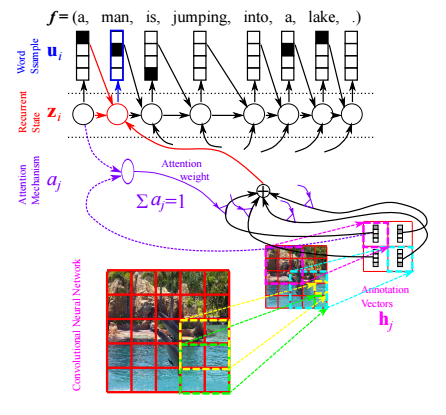
\includegraphics[scale=0.6]{Imgs/abedfw.png}
	\caption{ساختار چارچوب کاری ارائه شده در \cite{cho2015describing} در حوزه تولید شرح متناظر تصویر}
	\label{fig:5-abedfw}
\end{figure}


%\section{جاسازی کلمات}


\section{جمع‌بندی}
در این بخش، پژوهش‌های ارائه‌شده پیشین در حوزه تولید خودکار شرح متناظر تصاویر را مرور نمودیم. مانند تمام مسائل دیگر موجود در حوزه هوش مصنوعی، بررسی روش‌های تولید خودکار شرح بر تصاویر را با بررسی عمل‌کرد مغز انسان در درک و توصیف تصاویر،‌ شروع کردیم. 
\\
مطابق‌ با نتایج آزمایشات انجام شده روی مغز انسان، مغز ما قادر است در کمتر از 200 تا 500 میلی‌ثانیه، تمام اطلاعات مورد نیاز برای توصیف صحنه را از تصویر، استخراج نماید. در حالتی‌که اطلاعات مورد نیاز، به شکل ساختاربندی شده و در قالب فرم‌های پرسش‌نامه، جمع‌آوری شوند، قدرت بازیابی مغز به مراتب بیشتر از حالتی است که فرد ملزم به توصیف صحنه در چارچوب جملات باشد. با این مقدمه، می‌توان دریافت، فرایند درک صحنه، باید به مراتب سریع‌تر از فرایند تولید جمله، انجام شود.
\\
استفاده از مدل‌های گرافی احتمالی، در سال‌های قبل از 2014، روش اصلی و اساسی در درک صحنه و استخراج اطلاعات مورد نیاز از تصاویر، به حساب می‌آمد. مدل‌های استاندارد مختلفی در بین پژوهش‌های انجام شده در این حوزه به چشم می‌خورد. در این بین، نمونه‌هایی از مدل‌های میدان تصادفی مارکف، میدان تصادفی شرطی و مدل‌های مولد خاص‌منظوره طراحی شده توسط پژوهش‌گران را مورد بررسی قرار دادیم.
\\
از اواخر سال 2013، روش‌های مبتنی یادگیری عمیق، نظر بسیاری از پژوهش‌گرانی را که در حوزه تولید شرح متناظر تصویر فعالیت می‌کردند، به خود جلب نمودند. این دسته‌ از روش‌ها، به دلیل عمل‌کرد بهتری که از خود نشان دادند، توانستند جایگزین روش‌های گرافی احتمالاتی شوند. 
\\
از جمله پژوهش‌هایی که با استفاده از شبکه‌های عصبی عمیق اقدام به تولید شرح متناظر تصویر کردند، می‌توان به پژوهش خانم لی و همکارانش \cite{karpathy2015deep} در سال 2015  اشاره کرد. در مرحله آموزش این پژوهش، ابتدا با استفاده از روش شبکه عصبی کانولوشنی ناحیه‌ای که در بخش قبل، ارائه شد، نواحی تصویر که شامل تصویر یک جسم هستند، انتخاب شده و بردار ویژگی مربوط به هر کدام از این بخش‌ها، استخراج می‌شود.
\\
پس از این مرحله، بردار ویژگی مربوط به جملات موجود در مجموعه‌داده، توسط یک شبکه عصبی بازگشتی دوطرفه، استخراج می‌شود. برای این‌ کار، ابتدا بردار ویژگی مربوط به هر کلمه با استفاده از یک شبکه کلمه به بردار\lr{Word To Vec}، استخراج شده و به عنوان ورودی به شبکه بازگشتی دوطرفه داده می‌شوند. استفاده از شبکه بازگشتی دوطرفه این امکان را می‌دهد که تاثیر کلمات قبل و بعد از هر کلمه، در تولید بردار ویژگی جملات لحاظ شود.
\\
با بهینه‌سازی یک تابع انرژی روی این قسمت، شبکه عصبی بازگشتی دوطرفه و شبکه عصبی کانولوشنی با هم آموزش داده می‌شوند. از این طریق، بخش‌هایی از مدل که مربوط به تولید بردار ویژگی از جملات و استخراج نواحی تصاویر و بردار ویژگی مربوط به آن‌ها است، به طور کامل آموزش می‌بینند.
\\
در ادامه فرایند آموزش شبکه، با ارائه بردار ویژگی تولید شده توسط شبکه عصبی کانولوشنی آموزش دیده در بخش قبلی به یک شبکه عصبی بازگشتی دیگر، و ارائه جملات موجود در مجموعه‌داده به آن، شبکه عصبی بازگشتی را برای تولید جمله نهایی آموزش می‌دهیم.
\\
آزمایشات انجام شده روی این پژوهش، معیار \lr{BLEU} حاصل توسط روش را روی مجموعه‌داده \lr{MS COCO} در مقایسه با روش‌های دیگر ارزیابی کرده‌اند. در این آزمایشات، بهترین عمل‌کرد روش ارائه شده روی این مجموعه‌داده به امتیاز \lr{BLEU} برابر با 57.3 رسیده است و این در حالیست که روش \cite{mao2014explain} روی همان مجموعه‌داده به مقدار 55.0 رسیده است.
\\
یکی دیگر از روش‌های ارائه شده در این بخش، روشی است که در پژوهش \cite{chen2015mind} در سال 2015 ارائه شده است. در این روش، یک شبکه عصبی بازگشتی دوطرفه برای نگاشت جملات و تصاویر به یک‌دیگر استفاده شده است. مدل ارائه شده، قادر است با گرفتن تصویر به عنوان ورودی، شرح متناظر آن را در قالب یک جمله تولید و با گرفتن یک جمله به عنوان ورودی، تصویر مربوط به آن را با بازیابی نماید.
\\
در این روش با در نظر گرفتن واحد عصبی ارائه شده در پژوهش \cite{mikolov2010recurrent} و اضافه کردن دو متغیر دیگر به آن، مدل نهایی تولید شده است. متغیرهای اضافه شده به این مدل، شامل متغیری برای  بردار ویژگی تصویر و متغیر دیگر برای تفسیر بصری آخرین کلمه دیده شده، است.
\\
شبکه عصبی ارائه شده در این پژوهش، توزیع احتمال توام تصاویر و جملات را مدل‌سازی می‌نماید. در صورتی که جمله به عنوان ورودی داده شده باشد، توزیع احتمال تصویر به شرط جمله قابل محاسبه و تصویر مربوطه قابل بازیابی است. در صورتی‌که تصویر به عنوان ورودی داده شده باشد، توزیع احتمال جمله به شرط تصویر قابل محاسبه است.
\\
نتایج ارائه شده در این پژوهش، با روش‌های دیگر مقایسه شد. برای تولید جمله به شرط داشتن تصویر، میزان امتیاز \lr{BLEU} حاصل توسط مدل در بهترین حالت برای مجموعه‌داده \lr{Flickr8k} مقدار 13.1، برای مجموعه‌داده \lr{Flickr30k} مقدار 12.0 و برای مجموعه‌داده \lr{MS COCO} مقدار 18.8 بوده است. این در حالیست که نتایج حاصل برای مدل \lr{RNN + VGG} به ترتیب برابر با 12.4، 11.9 و 18.4 بوده و مقادیر به دست آمده برای جملاتی که توسط عوامل انسانی تولید شده‌اند به ترتیب برابر با 20.6، 18.9 و 19.2 بوده است. نتایج نشان می‌دهد، روش ارائه شده در حوزه تولید شرح متناظر تصاویر از روش‌های استاندارد دیگر بهتر بوده اما هنوز به جملات تولید شده توسط انسان نمی‌رسد.
\\
همین‌طور برای بازیابی تصاویر با داشتن جمله ورودی، نتایج حاصل توسط مدل برای مجموعه‌داده‌ \lr{Flickr30k} به ترتیب برای معیارهای \lr{R@1}، \lr{R@5}، \lr{R@10}  و \lr{Med r 500} در بهترین حالت برابر با 18.5، 45.7، 58.1 و 7 است. این در حالیست که نتایج حاصل توسط مدل \lr{RNN + VGG} به ترتیب برابر با 15.1، 41.1، 54.1 و 9 است.

چارچوب کاری رمزگذار-رمزگشا یکی از اصلی‌ترین چارچوب‌های کاری در حوزه ترجمه ماشینی و پیرو آن تولید شرح متناظر تصویر به شمار می‌رود. رمزگذار در این چارچوب کاری وظیفه نگاشت ورودی به فضای معنا و رمزگشا وظیفه نگاشت فضای معنا به فضای خروجی را بر عهده دارد. در حوزه ترجمه ماشینی معمولا از یک شبکه عصبی حافظه کوتاه‌مدت بلند به عنوان رمزگشا استفاده می‌شود. این شبکه عصبی با دریافت کلمات جمله ورودی به ترتیب، بردار حالت مخفی خود را به‌روز‌رسانی می‌نماید. در نهایت می‌توان از این بردار به عنوان بردار حاصل نگاشت جمله ورودی به فضای معنا استفاده نمود.
\\
رمزگشا در این چارچوب کاری با دریافت بردار ویژگی تولید شده توسط رمزگشا، عمل تولید خروجی را برعهده خواهد داشت. در حوزه ترجمه ماشینی معمولا یک شبکه عصبی بازگشتی برای رمزگشا می‌تواند مورد استفاده قرار بگیرد. به طور معمول، بردار ویژگی تولید شده توسط رمزگذار، به عنوان یک ورودی به رمزگشا داده می‌شود و رمزگشا در هر مرحله با تولید یک کلمه به عنوان خروجی، بردار حالت مخفی خود را به‌روزرسانی نموده و با استفاده از بردار حالت مخفی جدید، اقدام به تولید کلمه جدید می‌نماید.
\\
یکی از محدودیت‌های جدی فرایند مذکور این است که بردار ویژگی فقط یک بردار با طول ثابت است و اولا رمزگذار باید بتواند تمام اطلاعات قابل استخراج را تنها در این بردار جاسازی نماید و ثانیا رمزگشا باید بتواند تمام اطلاعات مورد نیاز خود برای تولید کلمه و جمله را فقط از همین یک بردار استخراج نماید. این مشکل، پژوهش‌گران را بر آن داشت تا بردار ویژگی را از یک بردار با طول ثابت به یک دنباله بردار با طول ثابت و تعداد متغیر تغییر دهند. 
\\
به بردارهای ویژگی تولید شده در حالت جدید، حاشیه‌نویسی می‌گویند. این حاشیه‌نویسی‌ها باید دارای دو شرط زیر باشند:
\begin{enumerate}
	\item دربرگیرنده تمام معنای ورودی باشند.
	\item تمرکز بیشتری روی معنای یک بخش مشخص از ورودی داشته باشند.
\end{enumerate}
با در نظر گرفتن این ویژگی‌ها، رمزگشا قادر خواهد بود تا هنگام تولید هر کلمه، روی معنای یک بخش از جمله تمرکز بیشتری داشته باشد و فقط از آن بخش برای تولید کلمه استفاده نماید. به این شکل، کلمات تولید شده شباهت بیشتری به ورودی خواهند داشت و ترجمه‌های بهتری حاصل خواهد شد. 
\\
در سال 2015، آقای بنجیو و همکارانش در پژوهش \cite{xu2015show} روشی ارائه دادند که در آن برای اولین بار از ایده استفاده از نقطه توجه در حوزه ترجمه ماشینی برای تولید شرح متناظر تصویر استفاده نمودند. در این پژوهش، از یک شبکه عصبی کانولوشنی به عنوان رمزگذار استفاده شده است. خروجی شبکه از لایه ماقبل آخر گرفته شده که منجر به ایجاد تعداد زیادی بردار ویژگی از تصویر می‌شود که هر کدام از این بردارهای ویژگی، از یک ناحیه از تصویر ایجاد شده‌اند و تمرکز بیشتری روی آن ناحیه داشته‌اند. 
\\
بدین ترتیب با استفاده از یک شبکه عصبی بازگشتی به عنوان رمزگشا و استفاده از بردارهای حاشیه‌نویسی ایجاد شده توسط رمزگذار می‌توان به راحتی عملیات تولید شرح متناظر تصویر را انجام داد. تنها نکته‌ای که باید مشخص شود، چگونگی استفاده از بردارهای حاشیه‌نویسی است. در این پژوهش دو روش مختلف برای استفاده از بردارهای حاشیه‌نویسی مطرح شده است.
\\
روش اول موسوم به روش توجه سخت، روشی است که در آن فقط یک بردار حاشیه‌نویسی انتخاب شده و از آن برای تولید جمله استفاده می‌شود. در این روش به هر یک از بردارهای حاشیه‌نویسی توسط یک مدل که قبلا آموزش دیده است، یک وزن اختصاص می‌دهیم و سپس با توجه به وزن‌های تخصیص داده شده به هر بردار حاشیه‌نویسی، یکی از آن‌ها را به عنوان بردار ویژگی تصویر انتخاب کرده و از آن در مراحل بعدی استفاده می‌کنیم.
\\
روش دوم موسوم به روش توجه نرم، روشی است که در آن یک بردار ویژگی کلی از روی بردارهای حاشیه‌نویسی تولید شده و از آن بردار در مراحل بعدی استفاده می‌شود. برای تولید این بردار نیز مانند روش توجه سخت، ابتدا توسط یک مدل که از پیش‌آموزش دیده است، به هر یک از بردارهای حاشیه‌نویسی یک وزن اختصاص می‌دهیم. سپس می‌توان با محاسبه امید ریاضی بردارهای حاشیه‌نویسی با توجه به وزن هر یک از آن‌ها بردار ویژگی نهایی را برای تصویر تولید و از آن برای تولید جمله استفاده کرد.
\\
آزمایشات انجام شده روی این مدل نشان می‌دهد، معیار \lr{BlEU-1} حاصل از این روش با استفاده از توجه سخت معمولا از مدل توجه نرم بیش‌تر بوده است. مطابق با نتایج گزارش شده در این پژوهش، میزان امتیاز \lr{BLEU-1} حاصل توسط توجه سخت روی مجموعه‌داده‌های \lr{MS COCO}، \lr{Flickr30k}  و \lr{Flickr8k} به ترتیب برابر با 71.8، 66.9 و 67.0 است. این در حالیست که امتیاز حاصل توسط توجه نرم روی همین مجموعه‌های داده، به ترتیب برابر با 70.8، 66.7 و 67.0 و امتیاز کسب شده توسط مدل \lr{Log Bilinear} در بهترین حالت، به ترتیب برابر با 70.8، 60.0 و 65.6 بوده است. 
\\
مطابق با آزمایشات انجام‌شده، استفاده از توجه نرم، معیار \lr{METEOR} را نسبت به استفاده از توجه سخت افزایش می‌دهد. طبق نتایج گزارش‌شده در پژوهش، امتیاز \lr{METEOR} حاصل از توجه نرم به ترتیب روی مجموعه‌داده‌های \lr{Flickr8k}، \lr{Flickr30k} و \lr{MS COCO} برابر با 18.93، 18.49 و 23.90 بوده است. این در حالیست که امتیاز کسب‌شده توسط توجه سخت به ترتیب برابر با 20.30، 18.46 و 23.04 و امتیاز کسب‌شده توسط روش \lr{Log Bilinear} در بهترین حالت به ترتیب برابر است با 17.31، 16.88 و 20.03. این موضوع نشان می‌دهد با وجود این‌که جملات تولید شده توسط روش توجه سخت با در نظر گرفتن جملات موجود در مجموعه‌داده از امتیاز بالاتری نسبت به جملات تولید شده توسط توجه نرم برخوردارند؛ استفاده از توجه نرم، منجر به تولید جملات قابل قبول‌تری توسط انسان می‌شود.
\\
پژوهش‌های مختلفی از این ایده در حوزه‌های مختلف استفاده نموده‌اند که گزارش مختصری از تعدادی از این پژوهش‌ها ارائه شده است.

